\renewcommand\thesection{A.\arabic{figure}}
\renewcommand\thefigure{\thesection.\arabic{figure}}
\renewcommand{\thetable}{A.\arabic{table}} 

\chapter*{ANEXO A: Resultados extendidos}
\label{ch:anexo}
\setcounter{figure}{0}
\setcounter{table}{0} 
En este capítulo se muestra el detalle numérico de las métricas componentes de $CMOPSO-CLAHE$. además de valores resultantes de las variables de decisión y tiempos de ejecución para las imágenes de prueba. para los resultados no dominados. Los tiempos de ejecución detallados corresponden a \texttt{time())} \cite{time}.

%Los resultados de este apartado son los promedios de los tiempos de ejecución. de los algoritmos \textit{Histogram Equalization} (HE). \textit{Multiscale Morphological Contrast Enhancement} (MMCE) y el algoritmo propuesto. para las 200 imágenes en escala de grises. Los algoritmos se implementaron con el framewok ImageJ y se hizo ejecutar 5 veces los experimentos. En la Tabla \ref{tabla22} se muestran los promedios de los tiempos de ejecución del algoritmo HE para las imágenes en escala de grises.

\section{Imagen de prueba \texttt{calhouse\_230.jpg}}

\scriptsize
\begin{longtable}{|c|c|c|c|c|c|c|c|}
% \centering
%\begin{tabular}
\hline
ID & $\mathscr{R}_x$ & $\mathscr{R}_y$ & $\mathscr{C}$ & $f_1(I.\vv{x})$ & $f_2(I.\vv{x})$ & $f_3(I.\vv{x})$ & $f_4(I.\vv{x})$ \\
0 & 23 & 3 & 57,3732575144 & 0,0292377 & 0,425724 & 0,412724 & 0,426577 \\
97 & 24 & 3 & 25,5610737092 & 0,0314603 & 0,420266 & 0,408046 & 0,421692 \\
145 & 17 & 3 & 54,6437033238 & 0,0318866 & 0,421223 & 0,40784 & 0,422096 \\
264 & 17 & 3 & 42,5351753326 & 0,0320687 & 0,421165 & 0,407786 & 0,422038 \\
597 & 15 & 3 & 37,8604544159 & 0,0324335 & 0,418419 & 0,405284 & 0,41951 \\
95 & 17 & 3 & 27,3747341617 & 0,0327239 & 0,417424 & 0,404622 & 0,418723 \\
384 & 15 & 3 & 34,674710421 & 0,0327873 & 0,417622 & 0,404595 & 0,418776 \\
897 & 16 & 3 & 31,9268872897 & 0,0329156 & 0,417416 & 0,40472 & 0,418845 \\
976 & 16 & 3 & 31,5996434554 & 0,0329747 & 0,417346 & 0,404664 & 0,418797 \\
173 & 15 & 3 & 30,4868378039 & 0,0330629 & 0,41647 & 0,403624 & 0,417737 \\
795 & 15 & 3 & 29,9099187121 & 0,0331659 & 0,416189 & 0,403386 & 0,417492 \\
216 & 15 & 3 & 27,1861226943 & 0,033587 & 0,414587 & 0,401996 & 0,416016 \\
41 & 12 & 3 & 0 & 0,0340767 & 0,413031 & 0,399763 & 0,414117 \\
191 & 12 & 3 & 38,2465814367 & 0,0345759 & 0,412369 & 0,399186 & 0,413501 \\
601 & 12 & 3 & 37,3130362909 & 0,034658 & 0,412267 & 0,3991 & 0,413406 \\
876 & 12 & 3 & 35,7290324923 & 0,0346832 & 0,412014 & 0,398878 & 0,413172 \\
271 & 12 & 3 & 28,5029445185 & 0,0361695 & 0,409605 & 0,396861 & 0,41102 \\
284 & 12 & 3 & 23,1372286768 & 0,036273 & 0,405213 & 0,393055 & 0,40713 \\
7 & 8 & 3 & 86,3634576987 & 0,0365424 & 0,401675 & 0,388628 & 0,402692 \\
873 & 8 & 3 & 33,7323253391 & 0,0368686 & 0,401169 & 0,388217 & 0,402252 \\
993 & 12 & 3 & 18,9568817854 & 0,0396409 & 0,398886 & 0,387114 & 0,40115 \\
715 & 8 & 3 & 19,8981950651 & 0,0398903 & 0,392763 & 0,380737 & 0,394642 \\
681 & 8 & 3 & 19,3046814893 & 0,0401602 & 0,391976 & 0,379959 & 0,393811 \\
182 & 8 & 3 & 18,4173409642 & 0,0407586 & 0,390247 & 0,378278 & 0,392203 \\
94 & 8 & 3 & 17,2658511178 & 0,0412259 & 0,387277 & 0,375334 & 0,389189 \\
155 & 8 & 3 & 16,8016243684 & 0,0418453 & 0,386054 & 0,374126 & 0,387956 \\
452 & 8 & 3 & 16,0485725832 & 0,0422859 & 0,383705 & 0,371776 & 0,385579 \\
590 & 8 & 3 & 15,2693772644 & 0,0425038 & 0,38073 & 0,368762 & 0,382451 \\
499 & 8 & 3 & 15,143110873 & 0,0434661 & 0,379937 & 0,367978 & 0,381609 \\
883 & 8 & 3 & 14,7557345894 & 0,0436602 & 0,378519 & 0,366529 & 0,380116 \\
558 & 8 & 3 & 14,6161046175 & 0,044045 & 0,377828 & 0,365838 & 0,379343 \\
393 & 8 & 3 & 14,5404305449 & 0,0456548 & 0,377069 & 0,365055 & 0,378529 \\
219 & 8 & 3 & 14,1441311249 & 0,0458689 & 0,375535 & 0,363518 & 0,376908 \\
158 & 8 & 3 & 14,0764285691 & 0,048008 & 0,374861 & 0,362849 & 0,376142 \\
877 & 8 & 3 & 13,7858094069 & 0,0481968 & 0,373455 & 0,361449 & 0,374686 \\
378 & 7 & 3 & 13,3843934032 & 0,0489759 & 0,37131 & 0,359071 & 0,372745 \\
261 & 7 & 3 & 13,3087797253 & 0,049448 & 0,370623 & 0,358357 & 0,371994 \\
169 & 7 & 3 & 13,0394378321 & 0,0503712 & 0,369149 & 0,356901 & 0,370396 \\
98 & 7 & 3 & 12,8029702226 & 0,0510101 & 0,368531 & 0,356287 & 0,369703 \\
498 & 7 & 3 & 12,6957022278 & 0,0528369 & 0,367707 & 0,355457 & 0,368871 \\
80 & 2 & 9 & 21,9803739685 & 0,0547318 & 0,370092 & 0,356346 & 0,365551 \\
571 & 2 & 9 & 20,4860987136 & 0,0552111 & 0,364453 & 0,350672 & 0,359591 \\
112 & 2 & 9 & 19,3139636962 & 0,0559449 & 0,360188 & 0,346436 & 0,355058 \\
595 & 2 & 9 & 19,0134812321 & 0,0573258 & 0,35901 & 0,345286 & 0,353856 \\
59 & 2 & 9 & 18,5934827218 & 0,058104 & 0,357468 & 0,343791 & 0,352303 \\
703 & 9 & 3 & 10,3704185678 & 0,058908 & 0,353311 & 0,341212 & 0,352759 \\
356 & 2 & 9 & 17,7548394545 & 0,0595813 & 0,353595 & 0,339995 & 0,348171 \\
684 & 2 & 9 & 17,3893954221 & 0,0602002 & 0,3522 & 0,338654 & 0,346685 \\
252 & 2 & 8 & 17,6230811316 & 0,0627446 & 0,351647 & 0,337268 & 0,345823 \\
257 & 2 & 8 & 16,7109381832 & 0,0634542 & 0,347473 & 0,333111 & 0,341571 \\
675 & 2 & 6 & 15,8882552359 & 0,0646944 & 0,338878 & 0,323731 & 0,333939 \\
171 & 2 & 6 & 15,1222111273 & 0,0647807 & 0,33565 & 0,320533 & 0,330537 \\
842 & 2 & 6 & 14,9422383356 & 0,0650434 & 0,334494 & 0,319402 & 0,329289 \\
226 & 2 & 6 & 14,1038613626 & 0,0651598 & 0,329654 & 0,314756 & 0,32418 \\
447 & 2 & 6 & 14,0672893813 & 0,0653296 & 0,329272 & 0,314427 & 0,323857 \\
79 & 2 & 6 & 13,8222357099 & 0,065599 & 0,327786 & 0,313001 & 0,322367 \\
267 & 2 & 6 & 13,6608515318 & 0,0656133 & 0,326686 & 0,311935 & 0,321176 \\
440 & 2 & 6 & 13,6386821722 & 0,0658236 & 0,326186 & 0,311441 & 0,320633 \\
194 & 2 & 6 & 13,4347941328 & 0,0669374 & 0,325037 & 0,31032 & 0,319386 \\
121 & 2 & 6 & 12,6219742475 & 0,067328 & 0,319971 & 0,305368 & 0,313821 \\
92 & 2 & 6 & 12,5297988526 & 0,0685897 & 0,319044 & 0,304494 & 0,312819 \\
251 & 2 & 6 & 12,1896188914 & 0,0698447 & 0,317086 & 0,302623 & 0,310927 \\
493 & 2 & 6 & 12,0368364323 & 0,070735 & 0,316246 & 0,301833 & 0,310161 \\
887 & 2 & 6 & 11,8321497111 & 0,07126 & 0,314152 & 0,299831 & 0,307934 \\
487 & 2 & 6 & 11,4967623408 & 0,0735698 & 0,311168 & 0,296897 & 0,304725 \\
542 & 5 & 3 & 7,67162409306 & 0,0749698 & 0,302866 & 0,290854 & 0,30122 \\
860 & 2 & 4 & 10,0745018143 & 0,0750613 & 0,293276 & 0,279185 & 0,290037 \\
539 & 2 & 6 & 8,79684436462 & 0,0769367 & 0,286597 & 0,272788 & 0,279622 \\
3 & 2 & 4 & 8,4270921169 & 0,0777197 & 0,276049 & 0,262486 & 0,271559 \\
514 & 2 & 4 & 8,40696827132 & 0,0793753 & 0,275258 & 0,26177 & 0,270849 \\
46 & 2 & 6 & 8,04438716466 & 0,0799718 & 0,277158 & 0,263589 & 0,269992 \\
102 & 2 & 6 & 7,9997365178 & 0,0802989 & 0,276266 & 0,262741 & 0,269098 \\
471 & 2 & 9 & 7,85180043792 & 0,0813022 & 0,275397 & 0,2635 & 0,269108 \\
1 & 2 & 5 & 7,96548201272 & 0,0814872 & 0,265061 & 0,252916 & 0,259859 \\
777 & 2 & 5 & 7,76557035058 & 0,0815563 & 0,262488 & 0,250409 & 0,257194 \\
405 & 2 & 5 & 7,68016122536 & 0,0819216 & 0,261172 & 0,249146 & 0,255847 \\
4 & 2 & 5 & 7,61629934678 & 0,082098 & 0,260247 & 0,24825 & 0,254892 \\
195 & 2 & 6 & 6,91195209853 & 0,0828915 & 0,25947 & 0,246359 & 0,252558 \\
234 & 2 & 5 & 7,48778556584 & 0,0837178 & 0,258099 & 0,246136 & 0,252683 \\
373 & 2 & 5 & 7,38351544203 & 0,0844555 & 0,257442 & 0,245512 & 0,252009 \\
387 & 2 & 6 & 6,78716478421 & 0,0847569 & 0,257979 & 0,244931 & 0,251067 \\
771 & 2 & 5 & 6,81921566464 & 0,0854425 & 0,250546 & 0,238638 & 0,245117 \\
407 & 2 & 3 & 5,43138516175 & 0,0869789 & 0,22301 & 0,212148 & 0,220494 \\
723 & 2 & 3 & 5,38666052144 & 0,0883751 & 0,222193 & 0,21133 & 0,219583 \\
140 & 2 & 3 & 5,13363566992 & 0,0900288 & 0,217382 & 0,206558 & 0,214437 \\
298 & 2 & 3 & 4,96763010595 & 0,0916071 & 0,214828 & 0,203994 & 0,211862 \\
319 & 2 & 3 & 4,85799070096 & 0,0932822 & 0,212195 & 0,201372 & 0,20903 \\
526 & 2 & 3 & 4,81280333702 & 0,0940423 & 0,210808 & 0,200041 & 0,207624 \\
45 & 2 & 3 & 4,79323134445 & 0,0968609 & 0,210167 & 0,199387 & 0,206933 \\
178 & 2 & 3 & 4,7385206072 & 0,0980654 & 0,209276 & 0,198493 & 0,205957 \\
10 & 2 & 3 & 4,57184432088 & 0,0981712 & 0,205247 & 0,194535 & 0,20186 \\
34 & 2 & 3 & 4,08287385715 & 0,0981765 & 0,193293 & 0,182853 & 0,189571 \\
992 & 2 & 3 & 4,01884732714 & 0,101047 & 0,19153 & 0,181147 & 0,187812 \\
396 & 2 & 3 & 3,9856954397 & 0,103705 & 0,189877 & 0,179515 & 0,1861 \\
722 & 2 & 3 & 3,95811781426 & 0,108743 & 0,188735 & 0,178423 & 0,184941 \\
743 & 2 & 3 & 3,85270193874 & 0,115116 & 0,184883 & 0,174711 & 0,181106 \\
43 & 2 & 3 & 3,63456542103 & 0,115272 & 0,177589 & 0,167514 & 0,173726 \\
82 & 2 & 3 & 3,54014931968 & 0,116835 & 0,174949 & 0,164953 & 0,171076 \\
103 & 2 & 3 & 3,49753256142 & 0,120246 & 0,172834 & 0,162913 & 0,168983 \\
228 & 2 & 3 & 3,42655439329 & 0,124204 & 0,170172 & 0,160381 & 0,166356 \\
89 & 2 & 3 & 3,39144518636 & 0,12493 & 0,168913 & 0,159211 & 0,165154 \\
77 & 2 & 3 & 3,32844054002 & 0,126974 & 0,164821 & 0,155251 & 0,1611 \\
506 & 2 & 3 & 3,28422335333 & 0,128863 & 0,163309 & 0,153766 & 0,159582 \\
73 & 2 & 3 & 3,25004004447 & 0,132968 & 0,161921 & 0,152441 & 0,158221 \\
127 & 2 & 3 & 3,22486879942 & 0,133743 & 0,160163 & 0,150728 & 0,156419 \\
17 & 2 & 3 & 3,15511690905 & 0,135205 & 0,158179 & 0,148785 & 0,154395 \\
106 & 2 & 3 & 3,11964708745 & 0,137987 & 0,15621 & 0,146931 & 0,152445 \\
131 & 2 & 3 & 3,03190160963 & 0,141845 & 0,151186 & 0,142191 & 0,147534 \\
86 & 2 & 3 & 2,9958936312 & 0,14586 & 0,149059 & 0,140118 & 0,145438 \\
747 & 2 & 3 & 2,95322617574 & 0,146119 & 0,147605 & 0,138739 & 0,144015 \\
78 & 2 & 3 & 2,89801274365 & 0,15009 & 0,145706 & 0,136892 & 0,142111 \\
72 & 2 & 3 & 2,75980332202 & 0,15052 & 0,138807 & 0,130323 & 0,135222 \\
42 & 2 & 3 & 2,67749869778 & 0,151622 & 0,134534 & 0,126169 & 0,130984 \\
122 & 2 & 3 & 2,64758257343 & 0,159517 & 0,133691 & 0,12534 & 0,130156 \\
57 & 2 & 3 & 2,59888888505 & 0,160515 & 0,132057 & 0,123734 & 0,128521 \\
138 & 2 & 3 & 2,55647560654 & 0,168326 & 0,130234 & 0,121997 & 0,126759 \\
68 & 2 & 3 & 2,5461703968 & 0,170373 & 0,128765 & 0,120523 & 0,125241 \\
55 & 2 & 3 & 2,45672191039 & 0,17349 & 0,124533 & 0,116481 & 0,121125 \\
411 & 2 & 3 & 2,43629302451 & 0,178669 & 0,122601 & 0,114592 & 0,119211 \\
23 & 2 & 3 & 2,37596020068 & 0,179921 & 0,120637 & 0,112692 & 0,117259 \\
84 & 2 & 3 & 2,36363878304 & 0,188776 & 0,11819 & 0,110339 & 0,11481 \\
19 & 2 & 3 & 2,27289241865 & 0,198626 & 0,113849 & 0,106283 & 0,110508 \\
16 & 2 & 3 & 2,18556239805 & 0,203667 & 0,110207 & 0,102788 & 0,106933 \\
156 & 2 & 4 & 2,10433011343 & 0,216118 & 0,10871 & 0,101138 & 0,10519 \\
85 & 2 & 3 & 2,13869778413 & 0,224032 & 0,106717 & 0,0993644 & 0,103488 \\
752 & 2 & 4 & 2,05457006729 & 0,228357 & 0,106082 & 0,0985937 & 0,10263 \\
185 & 4 & 3 & 1,92864636694 & 0,22998 & 0,105569 & 0,0977002 & 0,101977 \\
778 & 2 & 3 & 2,05250835305 & 0,234032 & 0,102608 & 0,0954123 & 0,0994415 \\
53 & 2 & 3 & 1,99410562164 & 0,234408 & 0,0996483 & 0,0925625 & 0,096537 \\
58 & 2 & 4 & 1,88120768276 & 0,240396 & 0,0963653 & 0,0894962 & 0,0931382 \\
25 & 2 & 3 & 1,80998124098 & 0,244 & 0,0905206 & 0,083824 & 0,0875545 \\
33 & 2 & 3 & 1,76706016276 & 0,258499 & 0,0886514 & 0,081945 & 0,0856682 \\
31 & 2 & 3 & 1,73836884281 & 0,264974 & 0,0864215 & 0,0797893 & 0,0834688 \\
69 & 2 & 3 & 1,6346154359 & 0,267809 & 0,0797979 & 0,0735224 & 0,0769657 \\
6 & 2 & 2 & 1,58883205633 & 0,287121 & 0,0769226 & 0,0706469 & 0,0743688 \\
671 & 2 & 2 & 1,58000196605 & 0,297476 & 0,0754181 & 0,0692956 & 0,0729723 \\
125 & 2 & 2 & 1,55504131254 & 0,300763 & 0,0734292 & 0,0672904 & 0,0708546 \\
52 & 2 & 3 & 1,49227705544 & 0,302547 & 0,071479 & 0,0655913 & 0,0687843 \\
128 & 2 & 3 & 1,44254540392 & 0,305737 & 0,0695817 & 0,0637585 & 0,0670127 \\
40 & 2 & 2 & 1,48516948564 & 0,312282 & 0,0694599 & 0,0635634 & 0,0670315 \\
47 & 2 & 3 & 1,42160592761 & 0,315582 & 0,065621 & 0,0601788 & 0,0631188 \\
38 & 2 & 3 & 1,32792087783 & 0,334522 & 0,0620888 & 0,0567531 & 0,0596328 \\
24 & 2 & 3 & 1,29923171946 & 0,341866 & 0,0589225 & 0,0539354 & 0,0566711 \\
37 & 2 & 3 & 1,27108655802 & 0,357528 & 0,0561818 & 0,051234 & 0,0539629 \\
21 & 2 & 3 & 1,20977573123 & 0,366692 & 0,0537357 & 0,0489777 & 0,0515024 \\
63 & 2 & 3 & 1,1432088483 & 0,379826 & 0,0495673 & 0,0451854 & 0,0476049 \\
51 & 2 & 3 & 1,11385295247 & 0,392391 & 0,0460724 & 0,042059 & 0,0443428 \\
83 & 2 & 3 & 1,07038368204 & 0,405484 & 0,0433605 & 0,0395519 & 0,041603 \\
497 & 2 & 3 & 1,03487871597 & 0,416443 & 0,0415171 & 0,0378856 & 0,0398424 \\
74 & 2 & 3 & 0,983928616331 & 0,422673 & 0,0391384 & 0,0356485 & 0,0375976 \\
28 & 2 & 3 & 0,962874904331 & 0,441196 & 0,0358967 & 0,0326292 & 0,0344847 \\
49 & 2 & 3 & 0,911749739956 & 0,452317 & 0,0334806 & 0,0305298 & 0,0321478 \\
64 & 2 & 3 & 0,886742609153 & 0,460282 & 0,0313939 & 0,0285593 & 0,0301892 \\
35 & 2 & 3 & 0,841926825957 & 0,472741 & 0,0288693 & 0,0262626 & 0,0277464 \\
296 & 2 & 2 & 0,850876965902 & 0,490974 & 0,0271727 & 0,0247413 & 0,0262711 \\
27 & 2 & 3 & 0,770359000241 & 0,494502 & 0,0247892 & 0,0225578 & 0,0238702 \\
48 & 2 & 3 & 0,728620775766 & 0,505156 & 0,0216592 & 0,0196863 & 0,0208914 \\
12 & 2 & 3 & 0,683879333277 & 0,516532 & 0,0201843 & 0,0183705 & 0,0194163 \\
13 & 2 & 3 & 0,647342056838 & 0,530366 & 0,0177617 & 0,0161534 & 0,0170947 \\
8 & 2 & 2 & 0,67282423446 & 0,555373 & 0,017341 & 0,0157395 & 0,0167658 \\
90 & 2 & 3 & 0,574015551604 & 0,567288 & 0,0141571 & 0,0127951 & 0,0135701 \\
62 & 2 & 3 & 0,559771230579 & 0,571877 & 0,0115625 & 0,0105159 & 0,011121 \\
196 & 2 & 3 & 0,510407911789 & 0,588363 & 0,0108908 & 0,00987159 & 0,0104669 \\
26 & 2 & 3 & 0,479204318984 & 0,59779 & 0,00906811 & 0,00822819 & 0,00867055 \\
748 & 2 & 6 & 0,506610195732 & 0,611275 & 0,00897331 & 0,00823064 & 0,00851013 \\
11 & 2 & 3 & 0,419813717968 & 0,614437 & 0,00742514 & 0,00670994 & 0,00714773 \\
720 & 2 & 3 & 0,398756230509 & 0,628389 & 0,00650833 & 0,00588966 & 0,00621115 \\
29 & 2 & 4 & 0,387786121852 & 0,631133 & 0,00581047 & 0,00528148 & 0,00556787 \\
197 & 2 & 2 & 0,357960602073 & 0,658577 & 0,00551113 & 0,00494194 & 0,00529456 \\
899 & 2 & 6 & 0,353321285556 & 0,66153 & 0,0046932 & 0,00427781 & 0,00440184 \\
279 & 3 & 4 & 0,3207766409 & 0,679144 & 0,00471416 & 0,00426083 & 0,00437535 \\
183 & 2 & 2 & 0,30109252741 & 0,682264 & 0,00351253 & 0,00309252 & 0,00331002 \\
60 & 2 & 3 & 0,237441707296 & 0,698645 & 0,00224598 & 0,00200366 & 0,00205784 \\
209 & 2 & 3 & 0,190721779561 & 0,708029 & 0,00164594 & 0,0014135 & 0,00148235 \\
797 & 2 & 4 & 0,172919850592 & 0,72584 & 0,00141331 & 0,00116224 & 0,00118492 \\
96 & 3 & 2 & 0,181018832469 & 0,747324 & 0,00127895 & 0,00107993 & 0,00111729 \\
585 & 7 & 2 & 0,0797504187823 & 0,750825 & 0,00109182 & 0,000858648 & 0,000898873 \\
295 & 2 & 4 & 0,141131526683 & 0,753901 & 0,000827484 & 0,000614913 & 0,000645663 \\
299 & 2 & 7 & 0,0924395774583 & 0,774405 & 0,000670587 & 0,000486303 & 0,000501837 \\
594 & 2 & 3 & 0,068058618312 & 0,775049 & 0,000299272 & 0,000143607 & 0,000141378 \\
30 & 2 & 2 & 0,00496512848939 & 0,788927 & 0,000204143 & 5,26E-05 & 5,18E-05 \\
\hline
\multicolumn{8}{|c|}{\textbf{Tiempos de ejecución:} \texttt{real:70m10.567s.user:207m55.583s.sys:95m37.939s}}\\  \hline
% \end{tabular}
\caption{Resultados no dominados para la imagen de prueba \texttt{calhouse\_230.jpg}}
\label{tab:calhouse_230}
\end{longtable}
\normalsize

\begin{figure}[H]
\centering
    %\begin{subfigure}[t]{0.45\textwidth}
    \begin{subfigure}[ID=0]{
    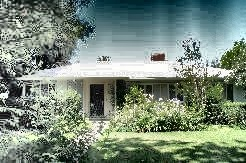
\includegraphics[width=0.45\textwidth]{./Figures/calhouse_230/0-resultado.jpg}
    }
%        \caption{Imagen Original. $\mathscr{H_Y}=0.207231$. $SSIM_R=1$. $SSIM_G=1$. $SSIM_B=1$}
\label{fig:calhouse2300}
\end{subfigure}
    ~ %add desired spacing between images. e. g. ~. \quad. \qquad. \hfill etc. 
      %(or a blank line to force the subfigure onto a new line)
      \begin{subfigure}[ID=1]{
      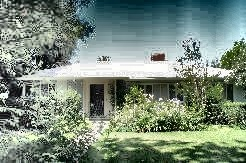
\includegraphics[width=0.45\textwidth]{./Figures/calhouse_230/1-resultado.jpg}   
      }
    %\begin{subfigure}[t]{0.45\textwidth}
%        \caption{Enhanced Image. $\mathscr{H_Y}=0.611275$. $SSIM_R=0.00897331$. $SSIM_G=0.00823064$. $SSIM_B=0.00851013$}
\label{fig:calhouse2301}
\end{subfigure}
    ~ %add desired spacing between images. e. g. ~. \quad. \qquad. \hfill etc. 
    %(or a blank line to force the subfigure onto a new line)
    \begin{subfigure}[ID=23]{
    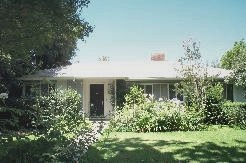
\includegraphics[width=0.45\textwidth]{./Figures/calhouse_230/23-resultado.jpg}
    }
    % \begin{subfigure}[t]{0.45\textwidth}
%        \caption{Enhanced Image.  $\mathscr{H_Y}=0.0350595$. $SSIM_R=0.416776$. $SSIM_G=0.403636$. $SSIM_B=0.417654$}
\label{fig:calhouse23023}
\end{subfigure} 
\begin{subfigure}[ID=24]{
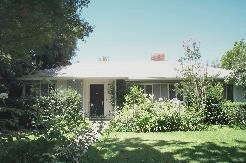
\includegraphics[width=0.45\textwidth]{./Figures/calhouse_230/24-resultado.jpg}
}
    % \begin{subfigure}[t]{0.45\textwidth}
        %\caption{Enhanced Image using \cite{morepso}. $\mathscr{H_Y}=0.788927$. $SSIM_R=0.000204143$. $SSIM_G=0.0000526475$. $SSIM_B=0.0000518143$}
        \label{fig:calhouse23024}
        \end{subfigure}
    ~ %add desired spacing between images. e. g. ~. \quad. \qquad. \hfill etc. 
    %(or a blank line to force the subfigure onto a new line)
    \begin{subfigure}[ID=56]{
    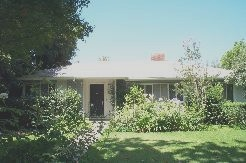
\includegraphics[width=0.45\textwidth]{./Figures/calhouse_230/56-resultado.jpg}
    }
    % \begin{subfigure}[t]{0.45\textwidth}
%        \caption{Enhanced Image.  $\mathscr{H_Y}=0.0350595$. $SSIM_R=0.416776$. $SSIM_G=0.403636$. $SSIM_B=0.417654$}
\label{fig:calhouse23056}
\end{subfigure} 
\begin{subfigure}[Imagen Original]{
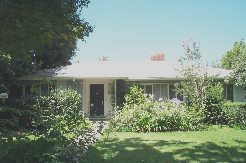
\includegraphics[width=0.45\textwidth]{./Figures/calhouse_230/calhouse_230.jpg}
}
    % \begin{subfigure}[t]{0.45\textwidth}
        %\caption{Enhanced Image using \cite{morepso}. $\mathscr{H_Y}=0.788927$. $SSIM_R=0.000204143$. $SSIM_G=0.0000526475$. $SSIM_B=0.0000518143$}
        \label{fig:calhouse230orig}
        \end{subfigure}
        \caption{Imágenes visualmente relevantes obtenidas mediante $CMOPSO-CLAHE$. Las variables y decisión y métricas de las imágenes se muestran en la tabla \ref{tab:calhouse_230}.}\label{fig:anexocalhouse230}
        \end{figure}

        \begin{figure}[H]
        \centering
        %\begin{subfigure}[Gráfica de Frente Pareto para las soluciones no dominadas de \texttt{calhouse_231.jpg}]{
        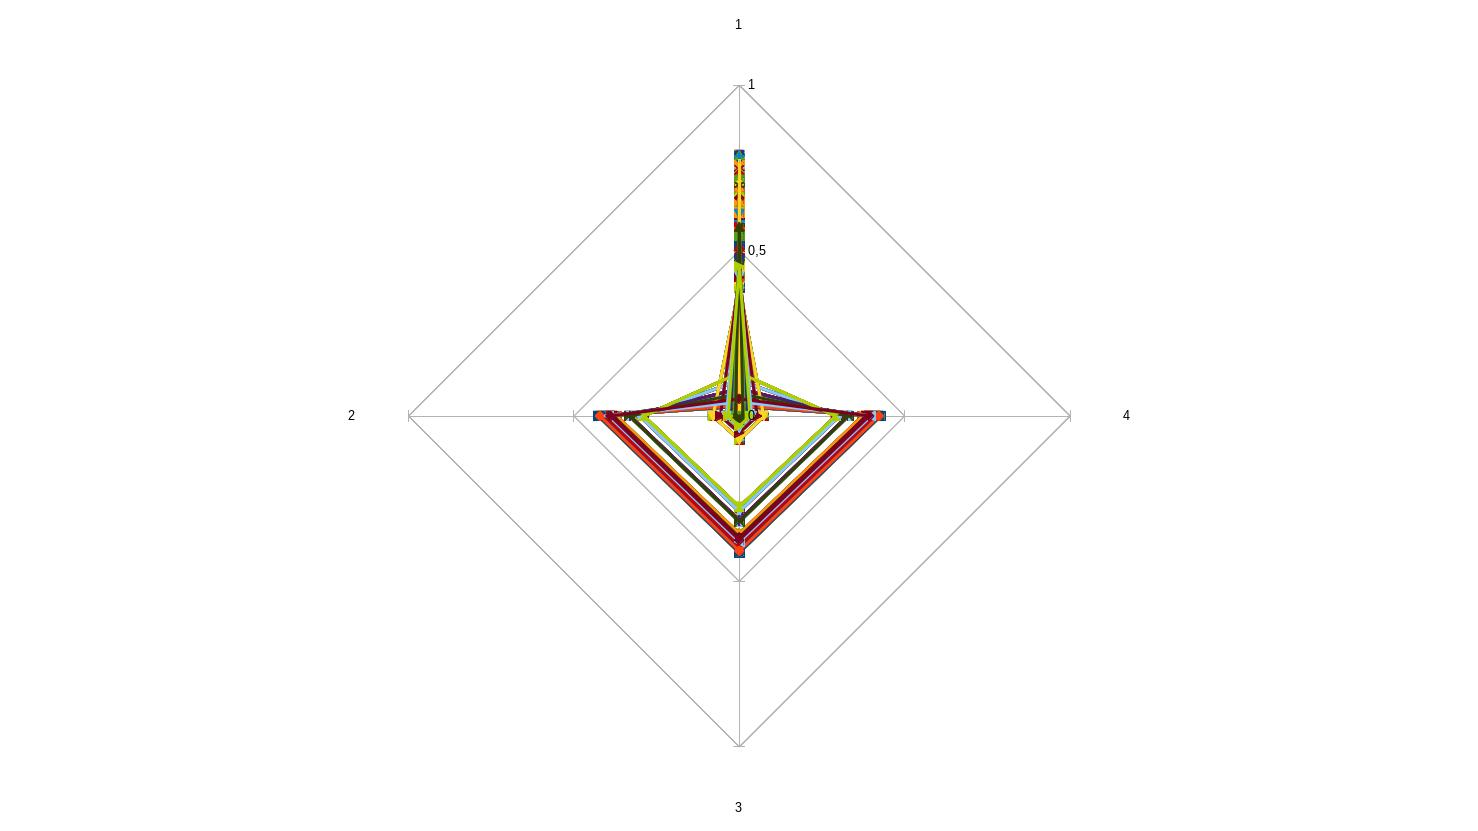
\includegraphics[width=\textwidth]{./Figures/calhouse_230/calhouse_230_2.jpg}
        %}
        %\end{subfigure}
        \caption{Frente pareto que contrasta los objetivos de las soluciones no dominadas. para los resultados de imágenes que se muestran en la tabla \ref{tab:calhouse_230}.}
        \label{fig:calhouse2302fp}
        \end{figure}


\section{Imagen de prueba \texttt{calhouse\_231.jpg}}

%calhouse 231
\scriptsize
\begin{longtable}{|c|c|c|c|c|c|c|c|}
% \centering
%\begin{tabular}
\hline
ID & $\mathscr{R}_x$ & $\mathscr{R}_y$ & $\mathscr{C}$ & $f_1(I.\vv{x})$ & $f_2(I.\vv{x})$ & $f_3(I.\vv{x})$ & $f_4(I.\vv{x})$ \\
0 & 2 & 2 & 0,528280568019 & 0,421322 & 0,011292 & 0,010746 & 0,0111554  \\
1 & 2 & 2 & 1 & 0,282013 & 0,038501 & 0,036779 & 0,0381451  \\
2 & 38 & 2 & 0 & 0,0125856 & 0,204869 & 0,200071 & 0,20363  \\
3 & 2 & 2 & 0 & 0,0431004 & 0,13865 & 0,136192 & 0,138648  \\
4 & 2 & 2 & 0,536034010196 & 0,41398 & 0,0131499 & 0,0124833 & 0,0130018  \\
5 & 2 & 2 & 0,198562769367 & 0,52922 & 0,00135061 & 0,00127997 & 0,00130769  \\
6 & 2 & 2 & 0,161635695061 & 0,540966 & 0,000784735 & 0,000735661 & 0,000749385  \\
7 & 2 & 2 & 0,00570221243692 & 0,573629 & 0,000103816 & 7,67837E-05 & 7,85741E-05  \\
8 & 3 & 2 & 0,716133888765 & 0,354162 & 0,0228098 & 0,0218175 & 0,0225493  \\
9 & 2 & 2 & 0,714396209779 & 0,359465 & 0,0228153 & 0,0216203 & 0,0225292  \\
10 & 3 & 2 & 0,593631709269 & 0,402347 & 0,0145436 & 0,0138748 & 0,0143605  \\
11 & 5 & 2 & 0,71780427577 & 0,3623 & 0,0212484 & 0,0204049 & 0,0209322  \\
12 & 17 & 2 & 0,699132537035 & 0,367131 & 0,0189012 & 0,0183635 & 0,0186746  \\
13 & 35 & 2 & 0,00864485180463 & 0,42346 & 0,0107601 & 0,0102734 & 0,0104956  \\
14 & 2 & 3 & 0,0577348012518 & 0,565069 & 0,000189286 & 0,000165373 & 0,000167802  \\
15 & 2 & 2 & 0,246783623874 & 0,513605 & 0,00194255 & 0,00184685 & 0,00190236  \\
16 & 10 & 2 & 0,888254299467 & 0,306106 & 0,0327387 & 0,0317938 & 0,032341  \\
17 & 8 & 2 & 0,811016594367 & 0,319267 & 0,0277445 & 0,0268512 & 0,0273699  \\
18 & 3 & 2 & 0,114333158176 & 0,549775 & 0,00055956 & 0,00050608 & 0,000516374  \\
19 & 8 & 2 & 0,492304222024 & 0,460667 & 0,00621708 & 0,00592585 & 0,00603826  \\
20 & 13 & 2 & 0 & 0,0130296 & 0,188019 & 0,183258 & 0,186758  \\
21 & 2 & 6 & 0,386888624299 & 0,471886 & 0,00573421 & 0,00559339 & 0,0057057  \\
22 & 4 & 2 & 0,579865472882 & 0,411112 & 0,013378 & 0,0127763 & 0,0131599  \\
23 & 9 & 2 & 1 & 0,298885 & 0,0334443 & 0,0324061 & 0,0330044  \\
24 & 5 & 2 & 0,834278139123 & 0,325659 & 0,0279524 & 0,0268406 & 0,0275564  \\
25 & 10 & 2 & 0,520833889993 & 0,428904 & 0,0107733 & 0,0101945 & 0,0103729  \\
26 & 8 & 2 & 0,624195274315 & 0,37555 & 0,0169599 & 0,0164014 & 0,016725  \\
27 & 3 & 2 & 0,627466735378 & 0,391768 & 0,0161627 & 0,0153941 & 0,0159548  \\
28 & 25 & 2 & 0,874755787269 & 0,372819 & 0,0186476 & 0,0180095 & 0,0183297  \\
29 & 2 & 2 & 0,870667176693 & 0,309887 & 0,0325293 & 0,0309195 & 0,0322076  \\
30 & 9 & 2 & 0,732234332042 & 0,365558 & 0,0191753 & 0,0185399 & 0,0188855  \\
31 & 2 & 2 & 0,444876042398 & 0,446127 & 0,00810596 & 0,00772429 & 0,00801587  \\
32 & 2 & 2 & 0,951954860788 & 0,289546 & 0,0364327 & 0,0347045 & 0,0360937  \\
33 & 19 & 2 & 1 & 0,271006 & 0,0385725 & 0,0376188 & 0,0381991  \\
34 & 19 & 2 & 0,618896353293 & 0,397269 & 0,0143794 & 0,0139211 & 0,0141685  \\
35 & 4 & 2 & 0,389600336216 & 0,475316 & 0,00536055 & 0,00515606 & 0,00529048  \\
36 & 10 & 2 & 0,425558569531 & 0,45027 & 0,00668378 & 0,00648114 & 0,00659949  \\
37 & 2605 & 2395 & 0,5 & 0,426877 & 0,0107589 & 0,0102665 & 0,0106218  \\
38 & 6 & 2 & 0,66522415478 & 0,383322 & 0,0160663 & 0,0154653 & 0,0158211  \\
39 & 7 & 2 & 0,599492521867 & 0,414094 & 0,0120755 & 0,0115387 & 0,0117838  \\
40 & 7 & 2 & 0,998931803013 & 0,276454 & 0,0381787 & 0,0368181 & 0,0376312  \\
41 & 8 & 2 & 0,771688109697 & 0,362255 & 0,0220707 & 0,0212203 & 0,0216666  \\
42 & 3 & 3 & 0,307589614694 & 0,49718 & 0,00289651 & 0,00277638 & 0,00282767  \\
43 & 13 & 2 & 0,944305010388 & 0,315595 & 0,029047 & 0,0281777 & 0,0286568  \\
44 & 5 & 2 & 0,966050230549 & 0,288689 & 0,0362972 & 0,0349026 & 0,0357714  \\
45 & 2 & 3 & 0,326108560547 & 0,491558 & 0,00390371 & 0,00373161 & 0,00387131  \\
46 & 2 & 3 & 0,15384887064 & 0,534519 & 0,00114637 & 0,00109067 & 0,00111032  \\
47 & 9 & 2 & 0,422208490979 & 0,462861 & 0,00579699 & 0,00562394 & 0,00572817  \\
48 & 7 & 2 & 0,497297664006 & 0,435993 & 0,00828631 & 0,00795353 & 0,00813127  \\
49 & 7 & 2 & 0,850549249493 & 0,328166 & 0,0265695 & 0,0256397 & 0,0261868  \\
50 & 2 & 4 & 0,223357597768 & 0,521675 & 0,00161956 & 0,00153988 & 0,00158018  \\
51 & 4 & 2 & 0,9930943249 & 0,284309 & 0,0371586 & 0,0357552 & 0,0367035  \\
52 & 12 & 2 & 1 & 0,307615 & 0,032043 & 0,0310592 & 0,0315852  \\
53 & 3 & 2 & 0,556872320691 & 0,414029 & 0,0125525 & 0,0119757 & 0,0123731  \\
54 & 2 & 3 & 0,0786234714955 & 0,561146 & 0,000201883 & 0,000166411 & 0,000174052  \\
55 & 3 & 2 & 0,421807093009 & 0,447001 & 0,00778622 & 0,00745209 & 0,00769754  \\
56 & 10 & 2 & 0 & 0,0134821 & 0,183211 & 0,178539 & 0,181995  \\
57 & 3 & 2 & 0,339142986519 & 0,47558 & 0,00452605 & 0,004307 & 0,00443858  \\
58 & 3 & 2 & 0 & 0,026926 & 0,160205 & 0,156303 & 0,159384  \\
59 & 6 & 2 & 0 & 0,0163016 & 0,174128 & 0,168903 & 0,172582  \\
60 & 5 & 2 & 0,364819047309 & 0,479774 & 0,00435225 & 0,00410036 & 0,00418851  \\
61 & 13 & 2 & 0,5 & 0,431454 & 0,00965356 & 0,00927182 & 0,0094467  \\
62 & 14 & 2 & 1 & 0,299743 & 0,0334014 & 0,0323744 & 0,0329796  \\
63 & 7 & 2 & 0 & 0,014287 & 0,177174 & 0,172057 & 0,1757  \\
64 & 3 & 3 & 0,0523409614263 & 0,573604 & 0,000167373 & 0,000136933 & 0,000144334  \\
65 & 4 & 3 & 0,228471662856 & 0,520381 & 0,00166707 & 0,00158428 & 0,0016109  \\
66 & 6 & 2 & 1 & 0,282743 & 0,0378731 & 0,0366182 & 0,0374679  \\
67 & 4 & 2 & 0,234783211652 & 0,516483 & 0,00166633 & 0,0015921 & 0,00162961  \\
68 & 20 & 2 & 1 & 0,270889 & 0,0385879 & 0,0376327 & 0,0382134  \\
69 & 6 & 3 & 0 & 0,0116286 & 0,242855 & 0,23726 & 0,242463  \\
70 & 3 & 2 & 0,206960598509 & 0,525156 & 0,00144721 & 0,00138333 & 0,00141691  \\
71 & 6 & 2 & 0,95332290819 & 0,295335 & 0,0347202 & 0,0334983 & 0,0342668  \\
72 & 18 & 2 & 0 & 0,012713 & 0,194229 & 0,189516 & 0,193111  \\
73 & 11 & 2 & 0 & 0,0133905 & 0,185665 & 0,180876 & 0,184348  \\
74 & 5 & 2 & 0,489580647303 & 0,442431 & 0,00817965 & 0,00780437 & 0,0080066  \\
75 & 4 & 2 & 0,30868061553 & 0,482928 & 0,00426761 & 0,00405113 & 0,00415045  \\
76 & 5 & 2 & 0 & 0,0177784 & 0,168074 & 0,162957 & 0,166491  \\
77 & 15 & 2 & 0,787845727898 & 0,338436 & 0,0232717 & 0,0226148 & 0,0229894  \\
78 & 7 & 2 & 0,255764762828 & 0,536006 & 0,00110823 & 0,00103223 & 0,00105307  \\
80 & 19 & 3 & 0 & 0,00900173 & 0,267205 & 0,261971 & 0,266923  \\
81 & 11 & 3 & 0 & 0,00997639 & 0,256986 & 0,251503 & 0,256516  \\
82 & 4 & 2 & 0 & 0,0226231 & 0,1636 & 0,159053 & 0,162368  \\
83 & 3 & 3 & 0,119503378494 & 0,546799 & 0,000724879 & 0,000653544 & 0,000674347  \\
84 & 4 & 2 & 0,286221733555 & 0,506126 & 0,00229212 & 0,00217746 & 0,00221458  \\
85 & 5 & 2 & 0,304026322185 & 0,506628 & 0,00222147 & 0,00211851 & 0,00215494  \\
86 & 2 & 7 & 0,0291606107902 & 0,551463 & 0,0005087 & 0,000484928 & 0,000491999  \\
87 & 3 & 2 & 0,31452246049 & 0,488762 & 0,00401598 & 0,00385289 & 0,00397122  \\
88 & 13 & 3 & 0 & 0,00985956 & 0,259264 & 0,253973 & 0,258887  \\
89 & 8 & 2 & 0,323020952705 & 0,475386 & 0,00529207 & 0,00510996 & 0,00520481  \\
90 & 3 & 2 & 0,950501160671 & 0,293769 & 0,0358847 & 0,0344679 & 0,0355097  \\
91 & 4 & 3 & 0,168281492455 & 0,530389 & 0,00119938 & 0,00115064 & 0,00116924  \\
92 & 3 & 2 & 0,79846119005 & 0,333691 & 0,0265783 & 0,0254337 & 0,0262778  \\
93 & 7 & 2 & 0,946888627685 & 0,312944 & 0,0307703 & 0,0297033 & 0,0303923  \\
94 & 9 & 3 & 0 & 0,0106044 & 0,253247 & 0,248009 & 0,252956  \\
95 & 8 & 3 & 0 & 0,0108852 & 0,248894 & 0,243521 & 0,248512  \\
96 & 5 & 2 & 0,204602199258 & 0,514978 & 0,00176819 & 0,00169965 & 0,00173187  \\
97 & 3 & 5 & 0,134621506197 & 0,55715 & 0,000453264 & 0,000428699 & 0,000432725  \\
98 & 6 & 2 & 0,441422354939 & 0,456932 & 0,00627423 & 0,00605903 & 0,00619215  \\
99 & 10 & 3 & 0 & 0,0104213 & 0,255358 & 0,250056 & 0,255104  \\
100 & 6 & 2 & 0,386927837815 & 0,456932 & 0,00627423 & 0,00605903 & 0,00619215  \\
101 & 2 & 2 & 0,451039281438 & 0,446127 & 0,00810596 & 0,00772429 & 0,00801587  \\
102 & 2 & 2 & 0 & 0,0431004 & 0,13865 & 0,136192 & 0,138648  \\
103 & 2 & 2 & 0,0445039999308 & 0,573629 & 0,000103816 & 7,67837E-05 & 7,85741E-05  \\
104 & 13 & 2 & 0,52911179301 & 0,431454 & 0,00965356 & 0,00927182 & 0,0094467  \\
105 & 2 & 2 & 1 & 0,282013 & 0,038501 & 0,036779 & 0,0381451  \\
106 & 10 & 2 & 0,905695427534 & 0,306106 & 0,0327387 & 0,0317938 & 0,032341  \\
107 & 6 & 2 & 0,976654715651 & 0,282743 & 0,0378731 & 0,0366182 & 0,0374679  \\
108 & 7 & 2 & 0,509946635219 & 0,435993 & 0,00828631 & 0,00795353 & 0,00813127  \\
109 & 5 & 2 & 0,970354083766 & 0,288689 & 0,0362972 & 0,0349026 & 0,0357714  \\
110 & 7 & 2 & 0 & 0,014287 & 0,177174 & 0,172057 & 0,1757  \\
\hline
\multicolumn{8}{|c|}{\textbf{Tiempos de ejecución:} \texttt{real:70m26.492s. user:209m3.921s. sys:95m37.357s}}\\  \hline
% \end{tabular}
\caption{Resultados no dominados para la imagen de prueba \texttt{calhouse\_231.jpg}}
\label{tab:calhouse_231}
\end{longtable}
\normalsize

\begin{figure}[H]
\centering
    %\begin{subfigure}[t]{0.45\textwidth}
    \begin{subfigure}[ID=0]{
    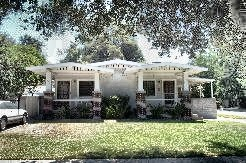
\includegraphics[width=0.45\textwidth]{./Figures/calhouse_231/0-resultado.jpg}
    }
%        \caption{Imagen Original. $\mathscr{H_Y}=0.207231$. $SSIM_R=1$. $SSIM_G=1$. $SSIM_B=1$}
\label{fig:calhouse2310}
\end{subfigure}
    ~ %add desired spacing between images. e. g. ~. \quad. \qquad. \hfill etc. 
      %(or a blank line to force the subfigure onto a new line)
      \begin{subfigure}[ID=1]{
      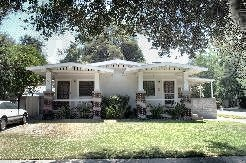
\includegraphics[width=0.45\textwidth]{./Figures/calhouse_231/1-resultado.jpg}   
      }
    %\begin{subfigure}[t]{0.45\textwidth}
%        \caption{Enhanced Image. $\mathscr{H_Y}=0.611275$. $SSIM_R=0.00897331$. $SSIM_G=0.00823064$. $SSIM_B=0.00851013$}
\label{fig:calhouse2311}
\end{subfigure}
    ~ %add desired spacing between images. e. g. ~. \quad. \qquad. \hfill etc. 
    %(or a blank line to force the subfigure onto a new line)
    \begin{subfigure}[ID=23]{
    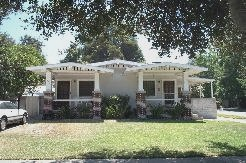
\includegraphics[width=0.45\textwidth]{./Figures/calhouse_231/28-resultado.jpg}
    }
    % \begin{subfigure}[t]{0.45\textwidth}
%        \caption{Enhanced Image.  $\mathscr{H_Y}=0.0350595$. $SSIM_R=0.416776$. $SSIM_G=0.403636$. $SSIM_B=0.417654$}
\label{fig:calhouse23128}
\end{subfigure} 
\begin{subfigure}[ID=24]{
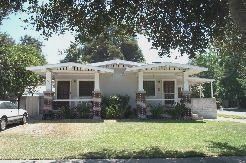
\includegraphics[width=0.45\textwidth]{./Figures/calhouse_231/29-resultado.jpg}
}
    % \begin{subfigure}[t]{0.45\textwidth}
        %\caption{Enhanced Image using \cite{morepso}. $\mathscr{H_Y}=0.788927$. $SSIM_R=0.000204143$. $SSIM_G=0.0000526475$. $SSIM_B=0.0000518143$}
        \label{fig:calhouse23129}
        \end{subfigure}
    ~ %add desired spacing between images. e. g. ~. \quad. \qquad. \hfill etc. 
    %(or a blank line to force the subfigure onto a new line)
    \begin{subfigure}[ID=56]{
    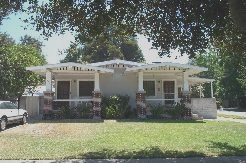
\includegraphics[width=0.45\textwidth]{./Figures/calhouse_231/102-resultado.jpg}
    }
    % \begin{subfigure}[t]{0.45\textwidth}
%        \caption{Enhanced Image.  $\mathscr{H_Y}=0.0350595$. $SSIM_R=0.416776$. $SSIM_G=0.403636$. $SSIM_B=0.417654$}
\label{fig:calhouse231102}
\end{subfigure} 
\begin{subfigure}[Imagen Original]{
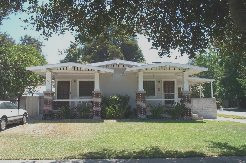
\includegraphics[width=0.45\textwidth]{./Figures/calhouse_231/calhouse_231.jpg}
}
    % \begin{subfigure}[t]{0.45\textwidth}
        %\caption{Enhanced Image using \cite{morepso}. $\mathscr{H_Y}=0.788927$. $SSIM_R=0.000204143$. $SSIM_G=0.0000526475$. $SSIM_B=0.0000518143$}
        \label{fig:calhouse231orig}
        \end{subfigure}
        \caption{Imágenes visualmente relevantes obtenidas mediante $CMOPSO-CLAHE$. Las variables y decisión y métricas de las imágenes se muestran en la tabla \ref{tab:calhouse_231}.}
        \label{fig:anexocalhouse230}
        \end{figure}

        \begin{figure}[H]
        \centering
        %\begin{subfigure}[Gráfica de Frente Pareto para las soluciones no dominadas de \texttt{calhouse_231.jpg}]{
        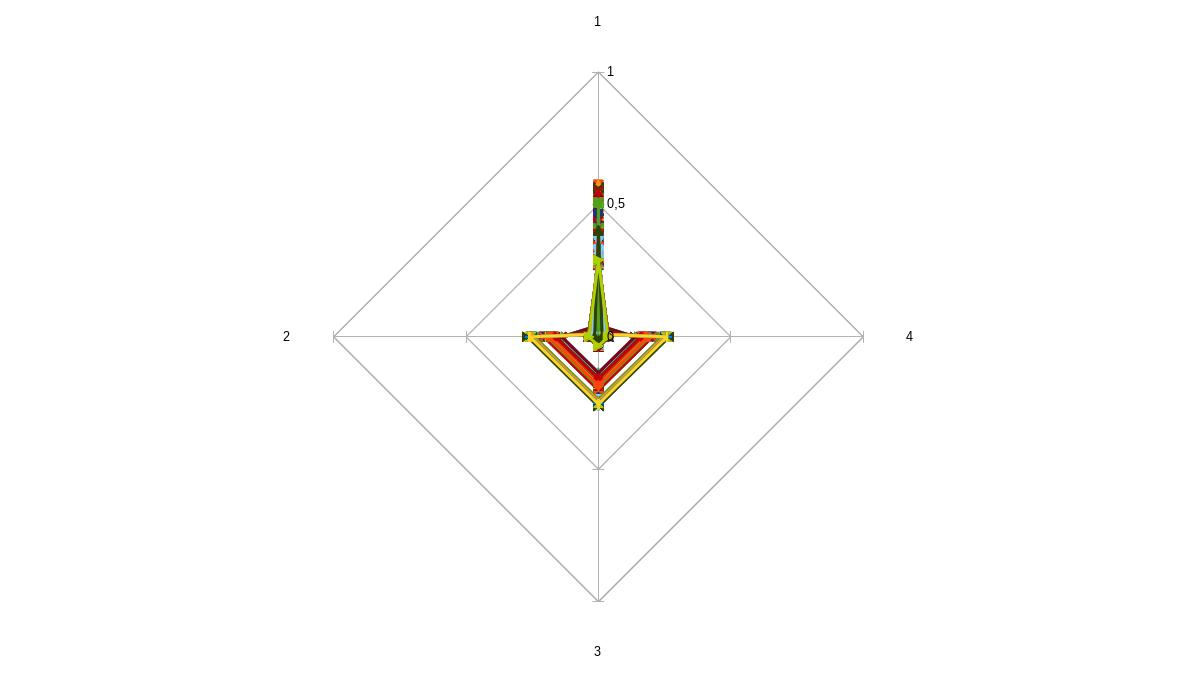
\includegraphics[width=\textwidth]{./Figures/calhouse_231/calhouse_231_2.jpg}
        %}
        %\end{subfigure}
        \caption{Frente pareto que contrasta los objetivos de las soluciones no dominadas. para los resultados de imágenes que se muestran en la tabla \ref{tab:calhouse_231}.}
        \label{fig:calhouse2312fp}
        \end{figure}

\section{Imagen de prueba \texttt{calhouse\_233.jpg}}

%calhouse 231
\scriptsize
\begin{longtable}{|c|c|c|c|c|c|c|c|}
% \centering
%\begin{tabular}
\hline
ID & $\mathscr{R}_x$ & $\mathscr{R}_y$ & $\mathscr{C}$ & $f_1(I.\vv{x})$ & $f_2(I.\vv{x})$ & $f_3(I.\vv{x})$ & $f_4(I.\vv{x})$ \\
0 & 2 & 3 & 0,295837914265 & 0,923925 & 0,00292607 & 0,00257795 & 0,00266449  \\
1 & 3 & 4 & 0,249135180036 & 0,92028 & 0,00292439 & 0,00261397 & 0,00266665  \\
2 & 4 & 3 & 0,214858343706 & 0,972543 & 0,00121931 & 0,00104515 & 0,00106603  \\
3 & 3 & 2 & 0 & 0,162343 & 0,36439 & 0,343949 & 0,35654  \\
4 & 2 & 2 & 0 & 0,166749 & 0,35221 & 0,33188 & 0,347256  \\
5 & 2 & 3 & 0,38662765211 & 0,864988 & 0,00550206 & 0,00480986 & 0,00499557  \\
6 & 2 & 2 & 0,00255100600277 & 1,09149 & 0,000183402 & 7,04854E-05 & 6,21437E-05  \\
7 & 5 & 2 & 0 & 0,0629735 & 0,391495 & 0,37163 & 0,381356  \\
8 & 2 & 4 & 0,618630059019 & 0,721047 & 0,0169986 & 0,0162408 & 0,0165372  \\
9 & 4 & 2 & 0 & 0,0834117 & 0,383713 & 0,363361 & 0,373847  \\
10 & 4 & 2 & 0,00239439320878 & 1,08964 & 0,000295689 & 0,000153393 & 0,000162248  \\
11 & 11 & 2 & 0 & 0,0619745 & 0,418598 & 0,398414 & 0,406889  \\
12 & 3 & 2 & 0,0778353881482 & 1,08786 & 0,000329964 & 0,000184893 & 0,000199624  \\
13 & 12 & 3 & 0,0239139002456 & 0,870766 & 0,00350392 & 0,00310311 & 0,00316902  \\
14 & 2 & 6 & 0,0389644204129 & 1,03646 & 0,000641662 & 0,000514385 & 0,000524924  \\
15 & 2 & 6 & 0 & 0,0455046 & 0,470176 & 0,461747 & 0,47771  \\
16 & 2 & 10 & 0 & 0,0359039 & 0,511722 & 0,502448 & 0,518851  \\
17 & 2 & 3 & 0,048680029034 & 1,05839 & 0,000302083 & 0,000187229 & 0,00018095  \\
18 & 8 & 3 & 0,0151713221581 & 1,03239 & 0,00102858 & 0,000843436 & 0,000877847  \\
19 & 2 & 3 & 0,184395984383 & 0,993392 & 0,00117745 & 0,00100106 & 0,00102251  \\
20 & 2 & 3 & 0,929331197893 & 0,664923 & 0,0280842 & 0,0260755 & 0,0268696  \\
21 & 40 & 4 & 0,466234114886 & 0,585286 & 0,0791404 & 0,0724312 & 0,0744605  \\
22 & 9 & 3 & 0 & 0,0462856 & 0,470122 & 0,456474 & 0,466522  \\
23 & 2 & 4 & 0,265528630888 & 0,919652 & 0,00348043 & 0,00316849 & 0,00322916  \\
24 & 5 & 3 & 0,5 & 0,810249 & 0,00887391 & 0,00800675 & 0,00821064  \\
25 & 2 & 4 & 0,822931346255 & 0,682197 & 0,0278131 & 0,0267008 & 0,0271825  \\
26 & 2 & 3 & 0,670636359678 & 0,758248 & 0,0146595 & 0,013324 & 0,0137805  \\
27 & 2 & 4 & 0,721496626868 & 0,697186 & 0,0211379 & 0,0202178 & 0,0205842  \\
28 & 2 & 4 & 0,578789027009 & 0,759783 & 0,0134854 & 0,0128619 & 0,0130943  \\
29 & 2 & 3 & 0,556768992896 & 0,798087 & 0,0102274 & 0,00910215 & 0,00944354  \\
30 & 2 & 9 & 0 & 0,0408697 & 0,499463 & 0,490757 & 0,507241  \\
31 & 6 & 3 & 0,757745094249 & 0,742439 & 0,016272 & 0,014948 & 0,0152924  \\
32 & 5 & 3 & 0,580904513711 & 0,785827 & 0,011758 & 0,0105297 & 0,010857  \\
33 & 2 & 3 & 1 & 0,638068 & 0,0319237 & 0,0297923 & 0,0307026  \\
34 & 2 & 4 & 0,76472395896 & 0,690287 & 0,0242775 & 0,023289 & 0,0236959  \\
35 & 2 & 3 & 0,621920299683 & 0,763786 & 0,0131498 & 0,0117422 & 0,0121901  \\
36 & 2 & 3 & 0,245737809351 & 0,95589 & 0,00235641 & 0,002009 & 0,00206351  \\
37 & 5 & 3 & 0,743495138096 & 0,75186 & 0,0155433 & 0,0142944 & 0,0146168  \\
38 & 8 & 3 & 0,5 & 0,819552 & 0,00842425 & 0,0076944 & 0,00785632  \\
39 & 2 & 4 & 0,37734382186 & 0,830931 & 0,00598392 & 0,00560268 & 0,0056997  \\
40 & 6 & 3 & 0 & 0,0475216 & 0,459573 & 0,445796 & 0,456496  \\
41 & 12 & 3 & 0,7551988051 & 0,715111 & 0,0179455 & 0,0167202 & 0,0170063  \\
42 & 43 & 3 & 0,517774282985 & 0,597537 & 0,0430642 & 0,0399363 & 0,0405722  \\
43 & 3 & 3 & 0,890204069895 & 0,694649 & 0,024789 & 0,0230342 & 0,0236651  \\
44 & 24 & 3 & 0,0161818033484 & 0,745152 & 0,0156444 & 0,0140341 & 0,0143124  \\
45 & 2 & 4 & 0,544526000725 & 0,778071 & 0,0115198 & 0,0108465 & 0,0110746  \\
46 & 3 & 4 & 0,534810140769 & 0,770255 & 0,0127545 & 0,0120351 & 0,0122763  \\
47 & 8 & 3 & 0,920940317282 & 0,682212 & 0,027619 & 0,026095 & 0,0265493  \\
48 & 11 & 3 & 0 & 0,0443048 & 0,475939 & 0,462247 & 0,471704  \\
49 & 3 & 3 & 0,715853976382 & 0,740592 & 0,0161852 & 0,0148598 & 0,015301  \\
50 & 10 & 3 & 0,69733899482 & 0,753103 & 0,0148294 & 0,0134841 & 0,0137764  \\
51 & 16 & 3 & 0,0168842090118 & 0,826457 & 0,00687623 & 0,00604448 & 0,00619402  \\
52 & 27 & 2 & 0 & 0,0599365 & 0,437032 & 0,417224 & 0,424583  \\
53 & 3 & 3 & 0,902217373237 & 0,688406 & 0,027186 & 0,0254119 & 0,0260424  \\
54 & 2 & 5 & 0,269495632959 & 0,938972 & 0,00280239 & 0,00262648 & 0,0026463  \\
55 & 46 & 3 & 0,143991202349 & 0,597537 & 0,0430642 & 0,0399363 & 0,0405722  \\
56 & 24 & 3 & 0,170169909589 & 0,745152 & 0,0156444 & 0,0140341 & 0,0143124  \\
57 & 2 & 3 & 0,243769872469 & 0,95589 & 0,00235641 & 0,002009 & 0,00206351  \\
58 & 4 & 2 & 0,100252601793 & 1,08964 & 0,000295689 & 0,000153393 & 0,000162248  \\
59 & 2 & 3 & 0,269440484107 & 0,923925 & 0,00292607 & 0,00257795 & 0,00266449  \\
60 & 2 & 2 & 0 & 0,166749 & 0,35221 & 0,33188 & 0,347256  \\
61 & 2 & 3 & 0,000678839983702 & 1,05839 & 0,000302083 & 0,000187229 & 0,00018095  \\
62 & 5 & 2 & 0 & 0,0629735 & 0,391495 & 0,37163 & 0,381356  \\
63 & 11 & 2 & 0 & 0,0619745 & 0,418598 & 0,398414 & 0,406889  \\
64 & 2 & 2 & 0,0137941023249 & 1,09149 & 0,000183402 & 7,04854E-05 & 6,21437E-05  \\
65 & 2 & 6 & 0 & 0,0455046 & 0,470176 & 0,461747 & 0,47771  \\
66 & 2 & 9 & 0 & 0,0408697 & 0,499463 & 0,490757 & 0,507241  \\
67 & 2 & 4 & 0,385219809226 & 0,830931 & 0,00598392 & 0,00560268 & 0,0056997  \\
68 & 2 & 10 & 0 & 0,0359039 & 0,511722 & 0,502448 & 0,518851  \\
69 & 4 & 2 & 0 & 0,0834117 & 0,383713 & 0,363361 & 0,373847  \\
70 & 2 & 4 & 0,608920213197 & 0,721047 & 0,0169986 & 0,0162408 & 0,0165372  \\
71 & 2 & 6 & 0,028621417168 & 1,03646 & 0,000641662 & 0,000514385 & 0,000524924  \\
72 & 3 & 2 & 0 & 0,162343 & 0,36439 & 0,343949 & 0,35654  \\
73 & 26 & 2 & 0 & 0,0599365 & 0,437032 & 0,417224 & 0,424583  \\
74 & 2 & 4 & 0,571638357607 & 0,759783 & 0,0134854 & 0,0128619 & 0,0130943  \\
75 & 2 & 4 & 0,295806477535 & 0,919652 & 0,00348043 & 0,00316849 & 0,00322916  \\
76 & 2 & 3 & 0,619162564166 & 0,763786 & 0,0131498 & 0,0117422 & 0,0121901  \\
77 & 11 & 3 & 0 & 0,0443048 & 0,475939 & 0,462247 & 0,471704  \\
78 & 2 & 3 & 0,923012222054 & 0,664923 & 0,0280842 & 0,0260755 & 0,0268696  \\
79 & 38 & 4 & 0,331480387773 & 0,585286 & 0,0791404 & 0,0724312 & 0,0744605  \\
80 & 2 & 3 & 0,586610008172 & 0,787139 & 0,0119147 & 0,0107169 & 0,0111113  \\
81 & 2 & 3 & 0,53060297987 & 0,798087 & 0,0102274 & 0,00910215 & 0,00944354  \\
82 & 2 & 5 & 0,288960146772 & 0,938972 & 0,00280239 & 0,00262648 & 0,0026463  \\
83 & 16 & 3 & 0,546573397577 & 0,826457 & 0,00687623 & 0,00604448 & 0,00619402  \\
84 & 12 & 3 & 0,0599093328487 & 0,870766 & 0,00350392 & 0,00310311 & 0,00316902  \\
85 & 2 & 3 & 1 & 0,638068 & 0,0319237 & 0,0297923 & 0,0307026  \\
86 & 2 & 4 & 0,516903002911 & 0,778071 & 0,0115198 & 0,0108465 & 0,0110746  \\
87 & 3 & 4 & 0,300588244554 & 0,92028 & 0,00292439 & 0,00261397 & 0,00266665  \\
88 & 2 & 4 & 0,816027236114 & 0,682197 & 0,0278131 & 0,0267008 & 0,0271825  \\
89 & 2 & 3 & 0,388266931502 & 0,864988 & 0,00550206 & 0,00480986 & 0,00499557  \\
90 & 12 & 3 & 0,872070781736 & 0,715111 & 0,0179455 & 0,0167202 & 0,0170063  \\
91 & 2 & 3 & 0,15845824826 & 0,993392 & 0,00117745 & 0,00100106 & 0,00102251  \\
92 & 4 & 3 & 0,214639357232 & 0,972543 & 0,00121931 & 0,00104515 & 0,00106603  \\
93 & 8 & 3 & 0,0863610173808 & 1,03239 & 0,00102858 & 0,000843436 & 0,000877847  \\
94 & 5 & 3 & 0,5 & 0,810249 & 0,00887391 & 0,00800675 & 0,00821064  \\
95 & 3 & 2 & 0,0882649269638 & 1,08786 & 0,000329964 & 0,000184893 & 0,000199624  \\
96 & 2 & 3 & 0,673309867537 & 0,758248 & 0,0146595 & 0,013324 & 0,0137805  \\
97 & 3 & 3 & 0,675600484061 & 0,740592 & 0,0161852 & 0,0148598 & 0,015301  \\
98 & 2 & 4 & 0,715592882128 & 0,697186 & 0,0211379 & 0,0202178 & 0,0205842  \\
99 & 5 & 3 & 0,691433319604 & 0,75186 & 0,0155433 & 0,0142944 & 0,0146168  \\
100 & 2 & 4 & 0,781038459568 & 0,690287 & 0,0242775 & 0,023289 & 0,0236959  \\
101 & 10 & 3 & 0,669395730455 & 0,753103 & 0,0148294 & 0,0134841 & 0,0137764  \\
102 & 3 & 3 & 0,573629042383 & 0,791412 & 0,0117933 & 0,0106632 & 0,0109955  \\
103 & 7 & 3 & 0 & 0,054872 & 0,462664 & 0,448778 & 0,459163  \\
104 & 3 & 4 & 0,57587859188 & 0,770255 & 0,0127545 & 0,0120351 & 0,0122763  \\
105 & 8 & 3 & 0,462590720779 & 0,819552 & 0,00842425 & 0,0076944 & 0,00785632  \\
106 & 3 & 3 & 1 & 0,662133 & 0,0302244 & 0,0283526 & 0,0290769  \\
107 & 8 & 3 & 0 & 0,0524292 & 0,466468 & 0,452746 & 0,463048  \\
108 & 6 & 3 & 0,977038740921 & 0,688181 & 0,027246 & 0,025366 & 0,0259008  \\
109 & 6 & 3 & 0,775674597529 & 0,742439 & 0,016272 & 0,014948 & 0,0152924  \\
110 & 9 & 3 & 0 & 0,0462856 & 0,470122 & 0,456474 & 0,466522  \\
111 & 38 & 4 & 0,628700727825 & 0,585286 & 0,0791404 & 0,0724312 & 0,0744605  \\
112 & 2 & 3 & 1 & 0,638068 & 0,0319237 & 0,0297923 & 0,0307026  \\
113 & 46 & 3 & 0,583476418714 & 0,597537 & 0,0430642 & 0,0399363 & 0,0405722  \\
114 & 12 & 3 & 0,797834935051 & 0,715111 & 0,0179455 & 0,0167202 & 0,0170063  \\
115 & 2 & 3 & 0,528084525906 & 0,798087 & 0,0102274 & 0,00910215 & 0,00944354  \\
116 & 2 & 4 & 0,517088638415 & 0,778071 & 0,0115198 & 0,0108465 & 0,0110746  \\
117 & 2 & 2 & 0,0172455393781 & 1,09149 & 0,000183402 & 7,04854E-05 & 6,21437E-05  \\
118 & 2 & 3 & 0,642160540603 & 0,758248 & 0,0146595 & 0,013324 & 0,0137805  \\
119 & 2 & 5 & 0,264991284514 & 0,938972 & 0,00280239 & 0,00262648 & 0,0026463  \\
120 & 2 & 2 & 0 & 0,166749 & 0,35221 & 0,33188 & 0,347256  \\
121 & 2 & 4 & 0,649144466259 & 0,721047 & 0,0169986 & 0,0162408 & 0,0165372  \\
122 & 3 & 3 & 0,920362895033 & 0,688406 & 0,027186 & 0,0254119 & 0,0260424  \\
123 & 5 & 3 & 0,5 & 0,810249 & 0,00887391 & 0,00800675 & 0,00821064  \\
\hline
\multicolumn{8}{|c|}{\textbf{Tiempos de ejecución:} \texttt{real:67m22.885s.user:207m13.352s.sys:94m57.439s
}}\\  \hline
% \end{tabular}
\caption{Resultados no dominados para la imagen de prueba \texttt{calhouse\_233.jpg}}
\label{tab:calhouse_233}
\end{longtable}
\normalsize

\begin{figure}[H]
\centering
    %\begin{subfigure}[t]{0.45\textwidth}
    \begin{subfigure}[ID=0]{
    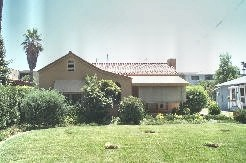
\includegraphics[width=0.45\textwidth]{./Figures/calhouse_233/6-resultado.jpg}
    }
%        \caption{Imagen Original. $\mathscr{H_Y}=0.207231$. $SSIM_R=1$. $SSIM_G=1$. $SSIM_B=1$}
\end{subfigure}
    ~ %add desired spacing between images. e. g. ~. \quad. \qquad. \hfill etc. 
      %(or a blank line to force the subfigure onto a new line)
      \begin{subfigure}[ID=1]{
      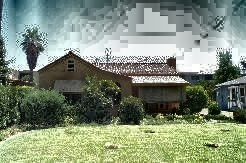
\includegraphics[width=0.45\textwidth]{./Figures/calhouse_233/7-resultado.jpg}   
      }
    %\begin{subfigure}[t]{0.45\textwidth}
%        \caption{Enhanced Image. $\mathscr{H_Y}=0.611275$. $SSIM_R=0.00897331$. $SSIM_G=0.00823064$. $SSIM_B=0.00851013$}
\end{subfigure}
    ~ %add desired spacing between images. e. g. ~. \quad. \qquad. \hfill etc. 
    %(or a blank line to force the subfigure onto a new line)
    \begin{subfigure}[ID=23]{
    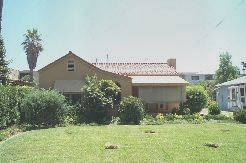
\includegraphics[width=0.45\textwidth]{./Figures/calhouse_233/46-resultado.jpg}
    }
    % \begin{subfigure}[t]{0.45\textwidth}
%        \caption{Enhanced Image.  $\mathscr{H_Y}=0.0350595$. $SSIM_R=0.416776$. $SSIM_G=0.403636$. $SSIM_B=0.417654$}
\end{subfigure} 
\begin{subfigure}[ID=24]{
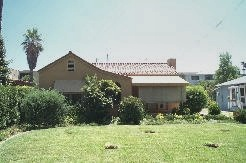
\includegraphics[width=0.45\textwidth]{./Figures/calhouse_233/47-resultado.jpg}
}
    % \begin{subfigure}[t]{0.45\textwidth}
        %\caption{Enhanced Image using \cite{morepso}. $\mathscr{H_Y}=0.788927$. $SSIM_R=0.000204143$. $SSIM_G=0.0000526475$. $SSIM_B=0.0000518143$}
        \label{fig:calhouse23129}
        \end{subfigure}
    ~ %add desired spacing between images. e. g. ~. \quad. \qquad. \hfill etc. 
    %(or a blank line to force the subfigure onto a new line)
    \begin{subfigure}[ID=56]{
    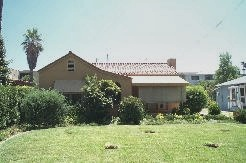
\includegraphics[width=0.45\textwidth]{./Figures/calhouse_233/60-resultado.jpg}
    }
    % \begin{subfigure}[t]{0.45\textwidth}
%        \caption{Enhanced Image.  $\mathscr{H_Y}=0.0350595$. $SSIM_R=0.416776$. $SSIM_G=0.403636$. $SSIM_B=0.417654$}
\label{fig:calhouse231102}
\end{subfigure} 
\begin{subfigure}[Imagen Original]{
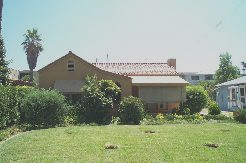
\includegraphics[width=0.45\textwidth]{./Figures/calhouse_233/calhouse_233.jpg}
}
    % \begin{subfigure}[t]{0.45\textwidth}
        %\caption{Enhanced Image using \cite{morepso}. $\mathscr{H_Y}=0.788927$. $SSIM_R=0.000204143$. $SSIM_G=0.0000526475$. $SSIM_B=0.0000518143$}
        \label{fig:calhouse233orig}
        \end{subfigure}
        \caption{Imágenes visualmente relevantes obtenidas mediante $CMOPSO-CLAHE$. Las variables y decisión y métricas de las imágenes se muestran en la tabla \ref{tab:calhouse_233}.}
        \label{fig:anexocalhouse233}
        \end{figure}

        \begin{figure}[H]
        \centering
        %\begin{subfigure}[Gráfica de Frente Pareto para las soluciones no dominadas de \texttt{calhouse_231.jpg}]{
        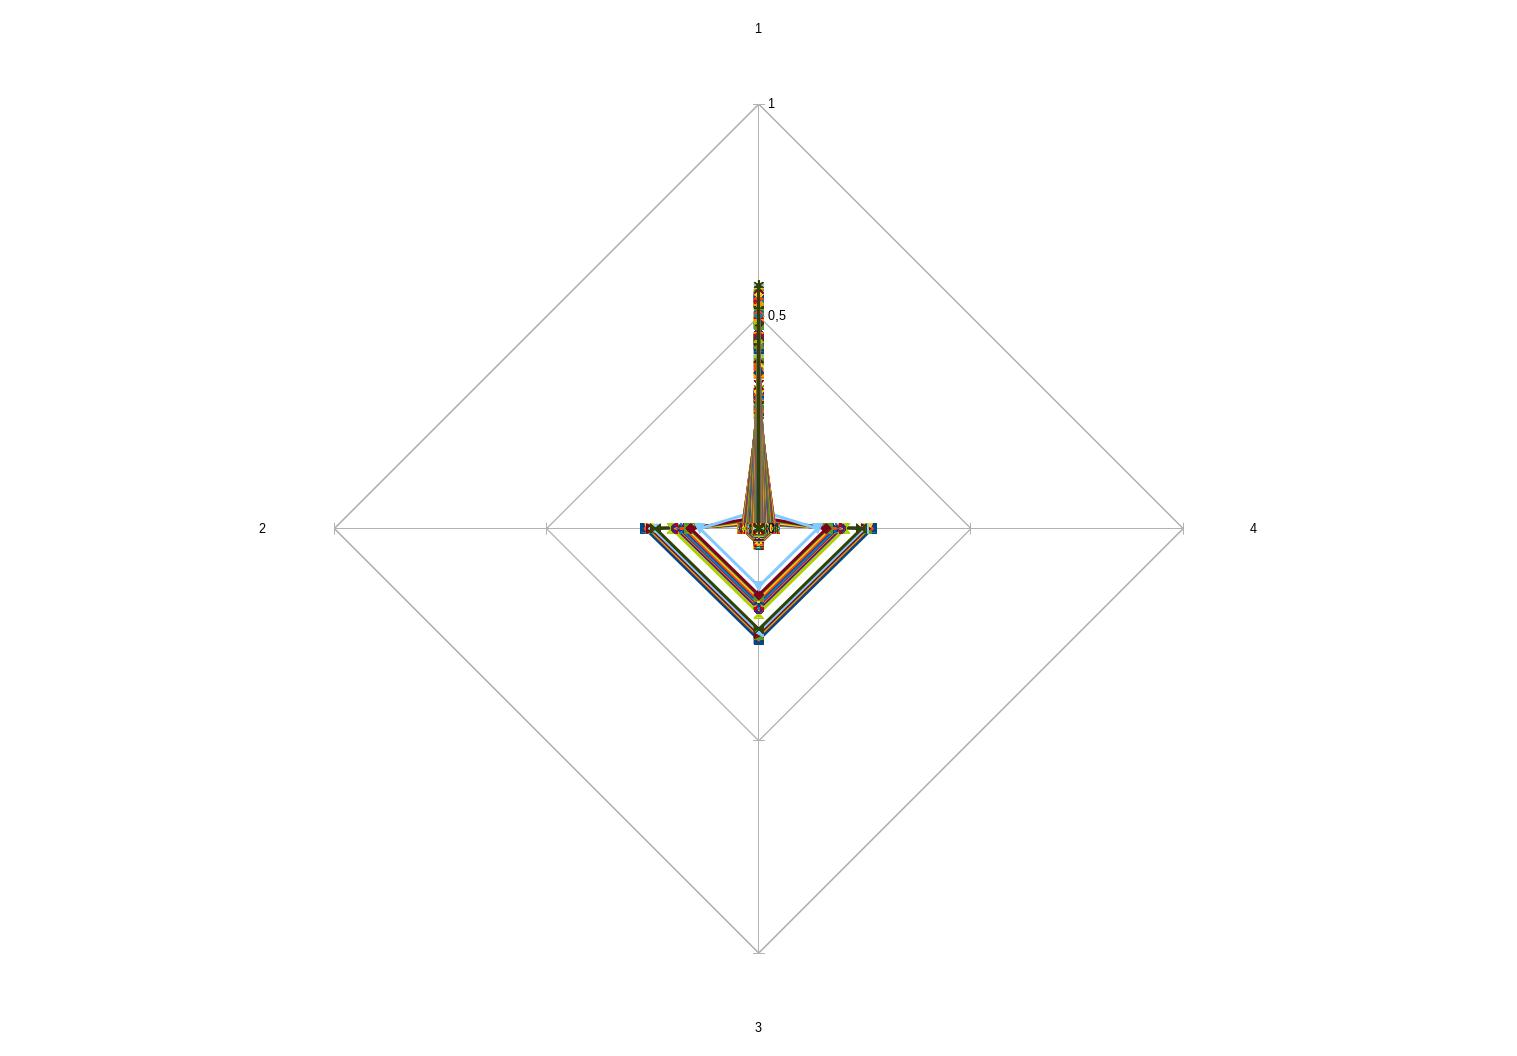
\includegraphics[width=\textwidth]{./Figures/calhouse_233/calhouse_233_2.jpg}
        %}
        %\end{subfigure}
        \caption{Frente pareto que contrasta los objetivos de las soluciones no dominadas. para los resultados de imágenes que se muestran en la tabla \ref{tab:calhouse_233}.}
        \label{fig:calhouse2332fp}
        \end{figure}


\section{Imagen de prueba \texttt{calhouse\_234.jpg}}

%calhouse 234
\scriptsize
\begin{longtable}{|c|c|c|c|c|c|c|c|}
% \centering
%\begin{tabular}
\hline
ID & $\mathscr{R}_x$ & $\mathscr{R}_y$ & $\mathscr{C}$ & $f_1(I.\vv{x})$ & $f_2(I.\vv{x})$ & $f_3(I.\vv{x})$ & $f_4(I.\vv{x})$ \\
0 & 3 & 2 & 0,818377249473 & 0,527355 & 0,0266691 & 0,0245697 & 0,0257519  \\
1 & 59 & 3 & 0,348404050444 & 0,41236 & 0,10348 & 0,0946411 & 0,0973958  \\
2 & 2 & 2 & 0,839606904816 & 0,515146 & 0,029663 & 0,0272264 & 0,0286435  \\
3 & 13 & 2 & 0,858950496855 & 0,524695 & 0,0260812 & 0,024745 & 0,0255167  \\
4 & 11 & 2 & 1 & 0,494054 & 0,034029 & 0,032038 & 0,0331011  \\
5 & 2 & 2 & 0,738264702174 & 0,548753 & 0,0229975 & 0,0211807 & 0,0222653  \\
6 & 27 & 6 & 0,665067465025 & 0,445776 & 0,0921568 & 0,0871899 & 0,0896835  \\
7 & 40 & 4 & 0,515435272603 & 0,445821 & 0,0866204 & 0,0792098 & 0,0816776  \\
8 & 3 & 3 & 0,802799465668 & 0,511109 & 0,0287218 & 0,0274117 & 0,0284403  \\
9 & 3 & 2 & 0,131123269978 & 0,793742 & 0,000731432 & 0,000664557 & 0,000679274  \\
10 & 10 & 2 & 0,707716171361 & 0,580588 & 0,0168114 & 0,0159317 & 0,0165228  \\
11 & 4 & 2 & 0,819304542919 & 0,519737 & 0,027535 & 0,0255765 & 0,0267492  \\
12 & 2 & 2 & 0 & 0,138669 & 0,231124 & 0,221532 & 0,228493  \\
13 & 18 & 2 & 0,5 & 0,62303 & 0,00889421 & 0,00828233 & 0,00854233  \\
14 & 14 & 2 & 0,973685974855 & 0,502234 & 0,0314391 & 0,0298899 & 0,0308901  \\
15 & 9 & 2 & 0,5 & 0,640419 & 0,00871692 & 0,00817691 & 0,00844283  \\
16 & 17 & 2 & 0,705975808503 & 0,574325 & 0,0167192 & 0,0159348 & 0,0164249  \\
17 & 8 & 2 & 0,376325532835 & 0,675727 & 0,00441494 & 0,00421142 & 0,00434589  \\
18 & 11 & 2 & 0,909204773465 & 0,513048 & 0,0288726 & 0,0272513 & 0,0282724  \\
19 & 12 & 2 & 0,5 & 0,601996 & 0,0103419 & 0,00983332 & 0,010186  \\
20 & 7 & 2 & 0 & 0,0413656 & 0,289774 & 0,282049 & 0,285934  \\
21 & 4 & 2 & 0,0881709349719 & 0,832464 & 0,000183395 & 0,000143403 & 0,000147903  \\
22 & 6 & 2 & 0,67190050469 & 0,564373 & 0,0195332 & 0,0183163 & 0,019096  \\
23 & 3 & 2 & 0,419925814383 & 0,664902 & 0,00713225 & 0,00668782 & 0,00695413  \\
24 & 4 & 2 & 0,293584223893 & 0,730788 & 0,00268251 & 0,00253008 & 0,00260924  \\
25 & 2 & 2 & 0,727267809131 & 0,553606 & 0,021385 & 0,0196689 & 0,0206698  \\
26 & 5 & 2 & 0,200766112685 & 0,738358 & 0,00171736 & 0,0016441 & 0,00168794  \\
27 & 11 & 2 & 0,35822182698 & 0,723333 & 0,00331185 & 0,00315496 & 0,00324682  \\
28 & 2 & 2 & 0,0155329642123 & 0,835548 & 0,000142314 & 0,000115598 & 0,000110237  \\
29 & 3 & 2 & 0,306795075516 & 0,710093 & 0,00364066 & 0,0034385 & 0,00355669  \\
30 & 2 & 3 & 0,893874350908 & 0,492458 & 0,0341363 & 0,0321934 & 0,0336531  \\
31 & 3 & 2 & 0,199177359771 & 0,755389 & 0,00142469 & 0,00136878 & 0,00139945  \\
32 & 6 & 2 & 0,769196682286 & 0,547824 & 0,0229913 & 0,0213657 & 0,0222196  \\
33 & 2 & 2 & 0,759973896268 & 0,54257 & 0,0246297 & 0,0226156 & 0,0237819  \\
34 & 2 & 2 & 0,91299851085 & 0,493326 & 0,0350073 & 0,032038 & 0,0337141  \\
35 & 6 & 2 & 0,185206673924 & 0,78611 & 0,000841764 & 0,00080091 & 0,000816869  \\
36 & 3 & 2 & 0 & 0,0846047 & 0,245215 & 0,237309 & 0,244065  \\
37 & 15 & 2 & 0,5 & 0,666303 & 0,00554846 & 0,00524035 & 0,00540413  \\
38 & 5 & 2 & 0,445174122796 & 0,66294 & 0,00827245 & 0,00775234 & 0,00802141  \\
39 & 7 & 2 & 0,236480112225 & 0,773407 & 0,00121588 & 0,00114323 & 0,00117378  \\
40 & 11 & 2 & 0 & 0,0396638 & 0,306313 & 0,297956 & 0,302221  \\
41 & 4 & 2 & 0,805472933679 & 0,530471 & 0,0249754 & 0,0230687 & 0,0241613  \\
42 & 24 & 2 & 0,950997765336 & 0,448877 & 0,0337654 & 0,0325268 & 0,0334449  \\
43 & 5 & 2 & 0 & 0,0519104 & 0,273498 & 0,265907 & 0,270653  \\
44 & 3 & 2 & 0,720115798569 & 0,551425 & 0,0215359 & 0,0198995 & 0,0208231  \\
45 & 6 & 2 & 0 & 0,0493283 & 0,277246 & 0,269315 & 0,27368  \\
46 & 3 & 3 & 0,634646330157 & 0,571977 & 0,0180757 & 0,0172713 & 0,0179017  \\
47 & 14 & 2 & 0,524848751778 & 0,58597 & 0,01286 & 0,0122675 & 0,0126854  \\
48 & 3 & 3 & 0,685028650384 & 0,553035 & 0,0211689 & 0,0201818 & 0,0209119  \\
49 & 3 & 2 & 0,463959307137 & 0,650707 & 0,00852852 & 0,00796836 & 0,00830184  \\
50 & 3 & 2 & 0,679025114903 & 0,557746 & 0,0203147 & 0,0187927 & 0,0196922  \\
51 & 23 & 3 & 0 & 0,0277634 & 0,406696 & 0,400567 & 0,40603  \\
52 & 7 & 3 & 0 & 0,0321503 & 0,363205 & 0,357271 & 0,362161  \\
53 & 19 & 3 & 0 & 0,0294476 & 0,401875 & 0,395903 & 0,401497  \\
54 & 3 & 2 & 0,0883240061534 & 0,829471 & 0,000258416 & 0,000220973 & 0,000231715  \\
55 & 2 & 3 & 0,105680467779 & 0,831217 & 0,000254231 & 0,000202246 & 0,000220666  \\
56 & 11 & 3 & 0 & 0,0296307 & 0,381211 & 0,374829 & 0,380207  \\
57 & 6 & 2 & 0,899388322835 & 0,496642 & 0,0326795 & 0,0303633 & 0,0316357  \\
58 & 4 & 2 & 0,864534440051 & 0,502655 & 0,0311266 & 0,0287067 & 0,03005  \\
59 & 2 & 3 & 0,050929948535 & 0,836594 & 0,000146742 & 0,000117982 & 0,000110062  \\
60 & 18 & 2 & 0,804145499558 & 0,533793 & 0,0238637 & 0,022623 & 0,0232914  \\
61 & 20 & 3 & 0 & 0,0284328 & 0,402012 & 0,396043 & 0,401629  \\
62 & 4 & 2 & 0,287960717289 & 0,730788 & 0,00268251 & 0,00253008 & 0,00260924  \\
63 & 2 & 2 & 0,0453845246446 & 0,835548 & 0,000142314 & 0,000115598 & 0,000110237  \\
64 & 7 & 2 & 0 & 0,0413656 & 0,289774 & 0,282049 & 0,285934  \\
65 & 2 & 2 & 0 & 0,138669 & 0,231124 & 0,221532 & 0,228493  \\
66 & 60 & 3 & 0,00140994587414 & 0,41236 & 0,10348 & 0,0946411 & 0,0973958  \\
67 & 7 & 3 & 0 & 0,0321503 & 0,363205 & 0,357271 & 0,362161  \\
68 & 5 & 2 & 0 & 0,0519104 & 0,273498 & 0,265907 & 0,270653  \\
69 & 7 & 2 & 0,206906460129 & 0,773407 & 0,00121588 & 0,00114323 & 0,00117378  \\
70 & 3 & 2 & 0,322271985499 & 0,710093 & 0,00364066 & 0,0034385 & 0,00355669  \\
71 & 2 & 3 & 0,029768001776 & 0,836594 & 0,000146742 & 0,000117982 & 0,000110062  \\
72 & 3 & 2 & 0 & 0,0846047 & 0,245215 & 0,237309 & 0,244065  \\
73 & 15 & 2 & 0,547945552478 & 0,666303 & 0,00554846 & 0,00524035 & 0,00540413  \\
74 & 3 & 2 & 0,0853731927042 & 0,829471 & 0,000258416 & 0,000220973 & 0,000231715  \\
75 & 2 & 2 & 0,72869127062 & 0,553606 & 0,021385 & 0,0196689 & 0,0206698  \\
76 & 3 & 2 & 0,136800145681 & 0,793742 & 0,000731432 & 0,000664557 & 0,000679274  \\
77 & 4 & 2 & 0,0163575505064 & 0,832464 & 0,000183395 & 0,000143403 & 0,000147903  \\
78 & 3 & 2 & 0,217635951343 & 0,755389 & 0,00142469 & 0,00136878 & 0,00139945  \\
79 & 18 & 2 & 0,636800145681 & 0,62303 & 0,00889421 & 0,00828233 & 0,00854233  \\
80 & 2 & 2 & 0,769040550106 & 0,54257 & 0,0246297 & 0,0226156 & 0,0237819  \\
81 & 8 & 2 & 0,323462111002 & 0,675727 & 0,00441494 & 0,00421142 & 0,00434589  \\
82 & 3 & 2 & 0,685598343219 & 0,557746 & 0,0203147 & 0,0187927 & 0,0196922  \\
83 & 17 & 2 & 0,645496357561 & 0,574325 & 0,0167192 & 0,0159348 & 0,0164249  \\
84 & 6 & 2 & 0 & 0,0493283 & 0,277246 & 0,269315 & 0,27368  \\
85 & 3 & 2 & 0,459463481702 & 0,650707 & 0,00852852 & 0,00796836 & 0,00830184  \\
86 & 11 & 2 & 0 & 0,0396638 & 0,306313 & 0,297956 & 0,302221  \\
87 & 20 & 3 & 0 & 0,0284328 & 0,402012 & 0,396043 & 0,401629  \\
88 & 36 & 4 & 0,277432850843 & 0,445821 & 0,0866204 & 0,0792098 & 0,0816776  \\
89 & 2 & 2 & 0,747676874116 & 0,548753 & 0,0229975 & 0,0211807 & 0,0222653  \\
90 & 14 & 2 & 1 & 0,502234 & 0,0314391 & 0,0298899 & 0,0308901  \\
91 & 12 & 2 & 0,5 & 0,601996 & 0,0103419 & 0,00983332 & 0,010186  \\
92 & 11 & 3 & 0 & 0,0296307 & 0,381211 & 0,374829 & 0,380207  \\
93 & 11 & 2 & 0,377393429315 & 0,723333 & 0,00331185 & 0,00315496 & 0,00324682  \\
94 & 2 & 3 & 0,893352619616 & 0,492458 & 0,0341363 & 0,0321934 & 0,0336531  \\
95 & 10 & 2 & 0,644314916717 & 0,580588 & 0,0168114 & 0,0159317 & 0,0165228  \\
96 & 24 & 2 & 1 & 0,448877 & 0,0337654 & 0,0325268 & 0,0334449  \\
97 & 14 & 2 & 0,537105312897 & 0,58597 & 0,01286 & 0,0122675 & 0,0126854  \\
98 & 11 & 2 & 1 & 0,494054 & 0,034029 & 0,032038 & 0,0331011  \\
99 & 2 & 2 & 0,835398992861 & 0,515146 & 0,029663 & 0,0272264 & 0,0286435  \\
100 & 4 & 2 & 0,898296732518 & 0,502655 & 0,0311266 & 0,0287067 & 0,03005  \\
101 & 18 & 2 & 0,793770605476 & 0,533793 & 0,0238637 & 0,022623 & 0,0232914  \\
102 & 9 & 2 & 0,514620698238 & 0,640419 & 0,00871692 & 0,00817691 & 0,00844283  \\
103 & 3 & 2 & 0,723171113862 & 0,551425 & 0,0215359 & 0,0198995 & 0,0208231  \\
104 & 6 & 2 & 0,671980206361 & 0,564373 & 0,0195332 & 0,0183163 & 0,019096  \\
105 & 4 & 2 & 0,816463208942 & 0,519737 & 0,027535 & 0,0255765 & 0,0267492  \\
106 & 2 & 2 & 0,929927397784 & 0,493326 & 0,0350073 & 0,032038 & 0,0337141  \\
107 & 23 & 3 & 0 & 0,0277634 & 0,406696 & 0,400567 & 0,40603  \\
108 & 13 & 3 & 0 & 0,0292034 & 0,390222 & 0,383769 & 0,389344  \\
109 & 5 & 2 & 0,231161071546 & 0,738358 & 0,00171736 & 0,0016441 & 0,00168794  \\
110 & 4 & 2 & 0,76242369505 & 0,530471 & 0,0249754 & 0,0230687 & 0,0241613  \\
\hline
\multicolumn{8}{|c|}{\textbf{Tiempos de ejecución:} \texttt{real:69m51.735s, user:207m51.484s, sys:94m33.030s}}\\  \hline
% \end{tabular}
\caption{Resultados no dominados para la imagen de prueba \texttt{calhouse\_234.jpg}}
\label{tab:calhouse_234}
\end{longtable}
\normalsize

\begin{figure}[H]
\centering
    %\begin{subfigure}[t]{0.45\textwidth}
    \begin{subfigure}[ID=0]{
    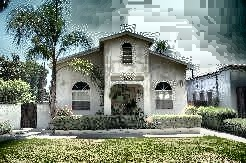
\includegraphics[width=0.45\textwidth]{./Figures/calhouse_234/1-resultado.jpg}
    }
%        \caption{Imagen Original. $\mathscr{H_Y}=0.207231$. $SSIM_R=1$. $SSIM_G=1$. $SSIM_B=1$}
\end{subfigure}
    ~ %add desired spacing between images. e. g. ~. \quad. \qquad. \hfill etc. 
      %(or a blank line to force the subfigure onto a new line)
      \begin{subfigure}[ID=1]{
      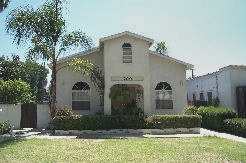
\includegraphics[width=0.45\textwidth]{./Figures/calhouse_234/2-resultado.jpg}   
      }
    %\begin{subfigure}[t]{0.45\textwidth}
%        \caption{Enhanced Image. $\mathscr{H_Y}=0.611275$. $SSIM_R=0.00897331$. $SSIM_G=0.00823064$. $SSIM_B=0.00851013$}
\end{subfigure}
    ~ %add desired spacing between images. e. g. ~. \quad. \qquad. \hfill etc. 
    %(or a blank line to force the subfigure onto a new line)
    \begin{subfigure}[ID=23]{
    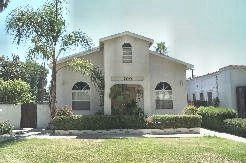
\includegraphics[width=0.45\textwidth]{./Figures/calhouse_234/51-resultado.jpg}
    }
    % \begin{subfigure}[t]{0.45\textwidth}
%        \caption{Enhanced Image.  $\mathscr{H_Y}=0.0350595$. $SSIM_R=0.416776$. $SSIM_G=0.403636$. $SSIM_B=0.417654$}
\end{subfigure} 
\begin{subfigure}[ID=24]{
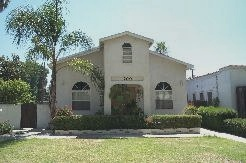
\includegraphics[width=0.45\textwidth]{./Figures/calhouse_234/59-resultado.jpg}
}
    % \begin{subfigure}[t]{0.45\textwidth}
        %\caption{Enhanced Image using \cite{morepso}. $\mathscr{H_Y}=0.788927$. $SSIM_R=0.000204143$. $SSIM_G=0.0000526475$. $SSIM_B=0.0000518143$}
        % \label{fig:calhouse23129}
        \end{subfigure}
    ~ %add desired spacing between images. e. g. ~. \quad. \qquad. \hfill etc. 
    %(or a blank line to force the subfigure onto a new line)
    \begin{subfigure}[ID=56]{
    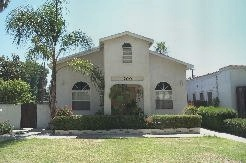
\includegraphics[width=0.45\textwidth]{./Figures/calhouse_234/60-resultado.jpg}
    }
    % \begin{subfigure}[t]{0.45\textwidth}
%        \caption{Enhanced Image.  $\mathscr{H_Y}=0.0350595$. $SSIM_R=0.416776$. $SSIM_G=0.403636$. $SSIM_B=0.417654$}
% \label{fig:calhouse231102}
\end{subfigure} 
\begin{subfigure}[Imagen Original]{
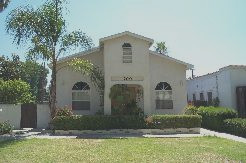
\includegraphics[width=0.45\textwidth]{./Figures/calhouse_234/calhouse_234.jpg}
}
    % \begin{subfigure}[t]{0.45\textwidth}
        %\caption{Enhanced Image using \cite{morepso}. $\mathscr{H_Y}=0.788927$. $SSIM_R=0.000204143$. $SSIM_G=0.0000526475$. $SSIM_B=0.0000518143$}
        % \label{fig:calhouse233orig}
        \end{subfigure}
        \caption{Imágenes visualmente relevantes obtenidas mediante $CMOPSO-CLAHE$. Las variables y decisión y métricas de las imágenes se muestran en la tabla \ref{tab:calhouse_234}.}
        \label{fig:anexocalhouse234}
        \end{figure}

        \begin{figure}[H]
        \centering
        %\begin{subfigure}[Gráfica de Frente Pareto para las soluciones no dominadas de \texttt{calhouse_231.jpg}]{
        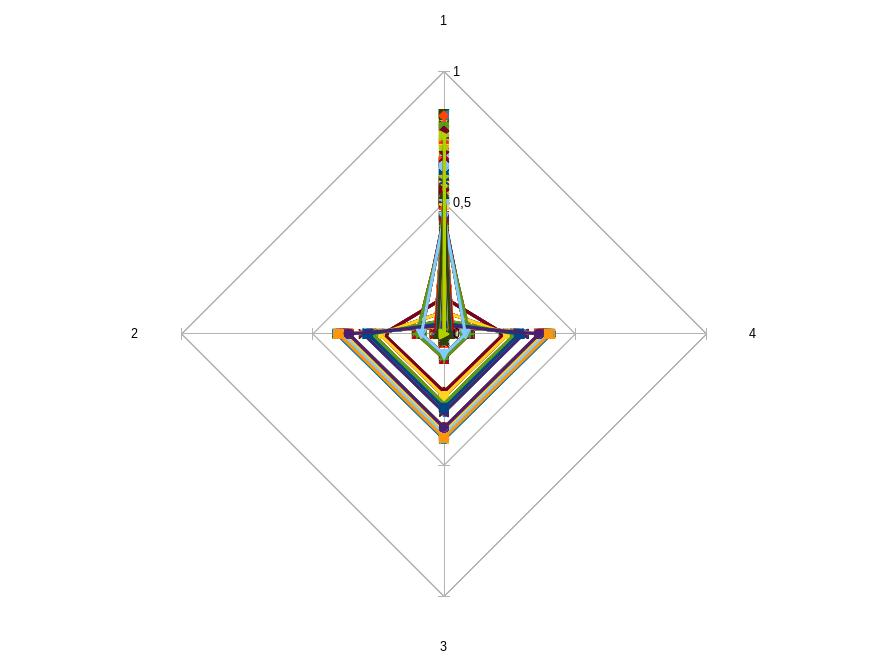
\includegraphics[width=\textwidth]{./Figures/calhouse_234/calhouse_234_2.jpg}
        %}
        %\end{subfigure}
        \caption{Frente pareto que contrasta los objetivos de las soluciones no dominadas. para los resultados de imágenes que se muestran en la tabla \ref{tab:calhouse_234}.}
        \label{fig:calhouse2342fp}
        \end{figure}


\section{Imagen de prueba \texttt{calhouse\_236.jpg}}

%calhouse 234
\scriptsize
\begin{longtable}{|c|c|c|c|c|c|c|c|}
% \centering
%\begin{tabular}
\hline
ID & $\mathscr{R}_x$ & $\mathscr{R}_y$ & $\mathscr{C}$ & $f_1(I.\vv{x})$ & $f_2(I.\vv{x})$ & $f_3(I.\vv{x})$ & $f_4(I.\vv{x})$ \\
\hline
0 & 3 & 2 & 0,818377249473 & 0,527355 & 0,0266691 & 0,0245697 & 0,0257519  \\
1 & 59 & 3 & 0,348404050444 & 0,41236 & 0,10348 & 0,0946411 & 0,0973958  \\
2 & 2 & 2 & 0,839606904816 & 0,515146 & 0,029663 & 0,0272264 & 0,0286435  \\
3 & 13 & 2 & 0,858950496855 & 0,524695 & 0,0260812 & 0,024745 & 0,0255167  \\
4 & 11 & 2 & 1 & 0,494054 & 0,034029 & 0,032038 & 0,0331011  \\
5 & 2 & 2 & 0,738264702174 & 0,548753 & 0,0229975 & 0,0211807 & 0,0222653  \\
6 & 27 & 6 & 0,665067465025 & 0,445776 & 0,0921568 & 0,0871899 & 0,0896835  \\
7 & 40 & 4 & 0,515435272603 & 0,445821 & 0,0866204 & 0,0792098 & 0,0816776  \\
8 & 3 & 3 & 0,802799465668 & 0,511109 & 0,0287218 & 0,0274117 & 0,0284403  \\
9 & 3 & 2 & 0,131123269978 & 0,793742 & 0,000731432 & 0,000664557 & 0,000679274  \\
10 & 10 & 2 & 0,707716171361 & 0,580588 & 0,0168114 & 0,0159317 & 0,0165228  \\
11 & 4 & 2 & 0,819304542919 & 0,519737 & 0,027535 & 0,0255765 & 0,0267492  \\
12 & 2 & 2 & 0 & 0,138669 & 0,231124 & 0,221532 & 0,228493  \\
13 & 18 & 2 & 0,5 & 0,62303 & 0,00889421 & 0,00828233 & 0,00854233  \\
14 & 14 & 2 & 0,973685974855 & 0,502234 & 0,0314391 & 0,0298899 & 0,0308901  \\
15 & 9 & 2 & 0,5 & 0,640419 & 0,00871692 & 0,00817691 & 0,00844283  \\
16 & 17 & 2 & 0,705975808503 & 0,574325 & 0,0167192 & 0,0159348 & 0,0164249  \\
17 & 8 & 2 & 0,376325532835 & 0,675727 & 0,00441494 & 0,00421142 & 0,00434589  \\
18 & 11 & 2 & 0,909204773465 & 0,513048 & 0,0288726 & 0,0272513 & 0,0282724  \\
19 & 12 & 2 & 0,5 & 0,601996 & 0,0103419 & 0,00983332 & 0,010186  \\
20 & 7 & 2 & 0 & 0,0413656 & 0,289774 & 0,282049 & 0,285934  \\
21 & 4 & 2 & 0,0881709349719 & 0,832464 & 0,000183395 & 0,000143403 & 0,000147903  \\
22 & 6 & 2 & 0,67190050469 & 0,564373 & 0,0195332 & 0,0183163 & 0,019096  \\
23 & 3 & 2 & 0,419925814383 & 0,664902 & 0,00713225 & 0,00668782 & 0,00695413  \\
24 & 4 & 2 & 0,293584223893 & 0,730788 & 0,00268251 & 0,00253008 & 0,00260924  \\
25 & 2 & 2 & 0,727267809131 & 0,553606 & 0,021385 & 0,0196689 & 0,0206698  \\
26 & 5 & 2 & 0,200766112685 & 0,738358 & 0,00171736 & 0,0016441 & 0,00168794  \\
27 & 11 & 2 & 0,35822182698 & 0,723333 & 0,00331185 & 0,00315496 & 0,00324682  \\
28 & 2 & 2 & 0,0155329642123 & 0,835548 & 0,000142314 & 0,000115598 & 0,000110237  \\
29 & 3 & 2 & 0,306795075516 & 0,710093 & 0,00364066 & 0,0034385 & 0,00355669  \\
30 & 2 & 3 & 0,893874350908 & 0,492458 & 0,0341363 & 0,0321934 & 0,0336531  \\
31 & 3 & 2 & 0,199177359771 & 0,755389 & 0,00142469 & 0,00136878 & 0,00139945  \\
32 & 6 & 2 & 0,769196682286 & 0,547824 & 0,0229913 & 0,0213657 & 0,0222196  \\
33 & 2 & 2 & 0,759973896268 & 0,54257 & 0,0246297 & 0,0226156 & 0,0237819  \\
34 & 2 & 2 & 0,91299851085 & 0,493326 & 0,0350073 & 0,032038 & 0,0337141  \\
35 & 6 & 2 & 0,185206673924 & 0,78611 & 0,000841764 & 0,00080091 & 0,000816869  \\
36 & 3 & 2 & 0 & 0,0846047 & 0,245215 & 0,237309 & 0,244065  \\
37 & 15 & 2 & 0,5 & 0,666303 & 0,00554846 & 0,00524035 & 0,00540413  \\
38 & 5 & 2 & 0,445174122796 & 0,66294 & 0,00827245 & 0,00775234 & 0,00802141  \\
39 & 7 & 2 & 0,236480112225 & 0,773407 & 0,00121588 & 0,00114323 & 0,00117378  \\
40 & 11 & 2 & 0 & 0,0396638 & 0,306313 & 0,297956 & 0,302221  \\
41 & 4 & 2 & 0,805472933679 & 0,530471 & 0,0249754 & 0,0230687 & 0,0241613  \\
42 & 24 & 2 & 0,950997765336 & 0,448877 & 0,0337654 & 0,0325268 & 0,0334449  \\
43 & 5 & 2 & 0 & 0,0519104 & 0,273498 & 0,265907 & 0,270653  \\
44 & 3 & 2 & 0,720115798569 & 0,551425 & 0,0215359 & 0,0198995 & 0,0208231  \\
45 & 6 & 2 & 0 & 0,0493283 & 0,277246 & 0,269315 & 0,27368  \\
46 & 3 & 3 & 0,634646330157 & 0,571977 & 0,0180757 & 0,0172713 & 0,0179017  \\
47 & 14 & 2 & 0,524848751778 & 0,58597 & 0,01286 & 0,0122675 & 0,0126854  \\
48 & 3 & 3 & 0,685028650384 & 0,553035 & 0,0211689 & 0,0201818 & 0,0209119  \\
49 & 3 & 2 & 0,463959307137 & 0,650707 & 0,00852852 & 0,00796836 & 0,00830184  \\
50 & 3 & 2 & 0,679025114903 & 0,557746 & 0,0203147 & 0,0187927 & 0,0196922  \\
51 & 23 & 3 & 0 & 0,0277634 & 0,406696 & 0,400567 & 0,40603  \\
52 & 7 & 3 & 0 & 0,0321503 & 0,363205 & 0,357271 & 0,362161  \\
53 & 19 & 3 & 0 & 0,0294476 & 0,401875 & 0,395903 & 0,401497  \\
54 & 3 & 2 & 0,0883240061534 & 0,829471 & 0,000258416 & 0,000220973 & 0,000231715  \\
55 & 2 & 3 & 0,105680467779 & 0,831217 & 0,000254231 & 0,000202246 & 0,000220666  \\
56 & 11 & 3 & 0 & 0,0296307 & 0,381211 & 0,374829 & 0,380207  \\
57 & 6 & 2 & 0,899388322835 & 0,496642 & 0,0326795 & 0,0303633 & 0,0316357  \\
58 & 4 & 2 & 0,864534440051 & 0,502655 & 0,0311266 & 0,0287067 & 0,03005  \\
59 & 2 & 3 & 0,050929948535 & 0,836594 & 0,000146742 & 0,000117982 & 0,000110062  \\
60 & 18 & 2 & 0,804145499558 & 0,533793 & 0,0238637 & 0,022623 & 0,0232914  \\
61 & 20 & 3 & 0 & 0,0284328 & 0,402012 & 0,396043 & 0,401629  \\
62 & 2 & 2 & 0,0609928161487 & 0,787766 & 0,000256124 & 0,000197123 & 0,000228562  \\
63 & 4 & 2 & 0,52223536612 & 0,569097 & 0,0147406 & 0,0145173 & 0,0152212  \\
64 & 9 & 2 & 0,505589934566 & 0,576457 & 0,014684 & 0,0144162 & 0,015154  \\
65 & 15 & 2 & 0,594417852291 & 0,523629 & 0,0229587 & 0,0225117 & 0,0233318  \\
66 & 3 & 2 & 0,716236838749 & 0,483283 & 0,0287522 & 0,027986 & 0,0294905  \\
67 & 2 & 2 & 0 & 0,0819087 & 0,255368 & 0,251915 & 0,257656  \\
68 & 3 & 2 & 0,269677482952 & 0,68885 & 0,00352479 & 0,00343585 & 0,00363311  \\
69 & 4 & 2 & 0,177913813107 & 0,737098 & 0,0013308 & 0,00132604 & 0,00137942  \\
70 & 3 & 2 & 0,256319244386 & 0,699975 & 0,00309802 & 0,00307773 & 0,00326212  \\
71 & 2 & 2 & 0,572082014846 & 0,566152 & 0,0173144 & 0,0169155 & 0,0180509  \\
72 & 17 & 2 & 0,501908060793 & 0,56284 & 0,0182472 & 0,017877 & 0,018825  \\
73 & 3 & 2 & 0,470797316063 & 0,601152 & 0,0117493 & 0,0114363 & 0,0120534  \\
74 & 2 & 2 & 0,28762897403 & 0,684397 & 0,00417191 & 0,00409187 & 0,00435506  \\
75 & 2 & 2 & 0,319001035677 & 0,676598 & 0,00467596 & 0,00454571 & 0,00490102  \\
76 & 2 & 2 & 0,0467344262764 & 0,791656 & 0,000155317 & 0,000121572 & 0,000128309  \\
77 & 2 & 2 & 0,806851045046 & 0,449825 & 0,0362412 & 0,0352132 & 0,0377132  \\
78 & 3 & 2 & 0,706400893583 & 0,496626 & 0,0260506 & 0,02529 & 0,0266687  \\
79 & 2 & 2 & 0,22026142931 & 0,724546 & 0,00201504 & 0,00198291 & 0,00209202  \\
80 & 3 & 2 & 0,134385763543 & 0,748132 & 0,00104085 & 0,000998748 & 0,00106332  \\
81 & 2 & 2 & 0,264811557652 & 0,697151 & 0,00318869 & 0,00307715 & 0,00330749  \\
82 & 2 & 2 & 0,789976935473 & 0,461123 & 0,0335764 & 0,032814 & 0,0350383  \\
83 & 2 & 2 & 0,132666358022 & 0,758529 & 0,000769288 & 0,000722369 & 0,000767623  \\
84 & 3 & 2 & 0,996037935634 & 0,384975 & 0,0502797 & 0,0486287 & 0,051306  \\
85 & 2 & 2 & 0,192442273151 & 0,728299 & 0,00148275 & 0,00144158 & 0,00152957  \\
86 & 2 & 2 & 0,721958245867 & 0,494555 & 0,0270831 & 0,0264682 & 0,0282887  \\
87 & 4 & 2 & 0,5 & 0,596839 & 0,0131762 & 0,0129074 & 0,0136321  \\
88 & 2 & 2 & 0,871233788733 & 0,431905 & 0,0403448 & 0,0392149 & 0,0419863  \\
89 & 2 & 2 & 0,384270287837 & 0,648621 & 0,007755 & 0,00755259 & 0,00805606  \\
90 & 41 & 4 & 0,863744583938 & 0,297561 & 0,107656 & 0,103902 & 0,105838  \\
91 & 3 & 2 & 0 & 0,0501919 & 0,282841 & 0,280242 & 0,285594  \\
92 & 4 & 2 & 0,229943686198 & 0,71229 & 0,00263194 & 0,00250156 & 0,00264687  \\
93 & 6 & 2 & 0,55477863176 & 0,564425 & 0,0178416 & 0,0174361 & 0,0182652  \\
94 & 3 & 2 & 0,940781652341 & 0,389108 & 0,0487418 & 0,0471518 & 0,0496774  \\
95 & 53 & 3 & 0,274034660606 & 0,276232 & 0,127112 & 0,120837 & 0,125981  \\
96 & 15 & 2 & 0,0848652779147 & 0,684746 & 0,00401761 & 0,00395017 & 0,00417073  \\
97 & 3 & 2 & 0,903800468918 & 0,409682 & 0,0439377 & 0,0424819 & 0,044889  \\
98 & 2 & 2 & 0,948583037555 & 0,407068 & 0,0475321 & 0,0460638 & 0,0492886  \\
99 & 3 & 2 & 0,0936325288752 & 0,777003 & 0,000383461 & 0,000322487 & 0,00035059  \\
100 & 2 & 2 & 0,0822339049711 & 0,775215 & 0,000484727 & 0,000458843 & 0,000490921  \\
101 & 3 & 2 & 0,669535264594 & 0,516613 & 0,0230328 & 0,0225424 & 0,0237412  \\
102 & 3 & 2 & 0,000663482307116 & 0,780215 & 0,0003251 & 0,000293507 & 0,000313995  \\
103 & 9 & 2 & 0,309579061915 & 0,671622 & 0,00477057 & 0,00471242 & 0,00498622  \\
104 & 4 & 2 & 0,905279192884 & 0,420893 & 0,0414817 & 0,0404199 & 0,0424878  \\
105 & 3 & 2 & 0,78506628645 & 0,46783 & 0,0316 & 0,0307277 & 0,0323041  \\
106 & 5 & 2 & 0,579659528424 & 0,542229 & 0,0191408 & 0,0188228 & 0,0197266  \\
107 & 5 & 2 & 0,696056694267 & 0,494868 & 0,0275482 & 0,0270448 & 0,0282753  \\
108 & 3 & 2 & 0,833889686802 & 0,434412 & 0,0382984 & 0,0371935 & 0,0391734  \\
109 & 3 & 2 & 0,5 & 0,578231 & 0,0139116 & 0,0136808 & 0,0144633  \\
110 & 4 & 2 & 0,41014792752 & 0,615799 & 0,0091199 & 0,00902098 & 0,00947175  \\
111 & 2 & 2 & 0,116924112842 & 0,767094 & 0,000488963 & 0,000461673 & 0,000486079  \\
\multicolumn{8}{|c|}{\textbf{Tiempos de ejecución:} \texttt{real:70m14.144s,user:208m40.536s,sys:94m45.105s
}}\\  \hline
% \end{tabular}
\caption{Resultados no dominados para la imagen de prueba \texttt{calhouse\_236.jpg}}
\label{tab:calhouse_236}
\end{longtable}
\normalsize

\begin{figure}[H]
\centering
    %\begin{subfigure}[t]{0.45\textwidth}
    \begin{subfigure}[ID=0]{
    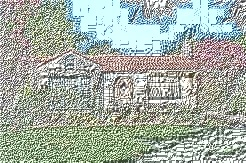
\includegraphics[width=0.45\textwidth]{./Figures/calhouse_236/56-resultado.jpg}
    }
%        \caption{Imagen Original. $\mathscr{H_Y}=0.207231$. $SSIM_R=1$. $SSIM_G=1$. $SSIM_B=1$}
\end{subfigure}
    ~ %add desired spacing between images. e. g. ~. \quad. \qquad. \hfill etc. 
      %(or a blank line to force the subfigure onto a new line)
      \begin{subfigure}[ID=1]{
      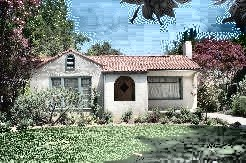
\includegraphics[width=0.45\textwidth]{./Figures/calhouse_236/61-resultado.jpg}   
      }
    %\begin{subfigure}[t]{0.45\textwidth}
%        \caption{Enhanced Image. $\mathscr{H_Y}=0.611275$. $SSIM_R=0.00897331$. $SSIM_G=0.00823064$. $SSIM_B=0.00851013$}
\end{subfigure}
    ~ %add desired spacing between images. e. g. ~. \quad. \qquad. \hfill etc. 
    %(or a blank line to force the subfigure onto a new line)
    \begin{subfigure}[ID=23]{
    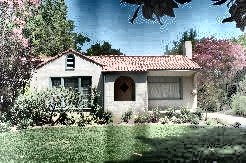
\includegraphics[width=0.45\textwidth]{./Figures/calhouse_236/82-resultado.jpg}
    }
    % \begin{subfigure}[t]{0.45\textwidth}
%        \caption{Enhanced Image.  $\mathscr{H_Y}=0.0350595$. $SSIM_R=0.416776$. $SSIM_G=0.403636$. $SSIM_B=0.417654$}
\end{subfigure} 
\begin{subfigure}[ID=24]{
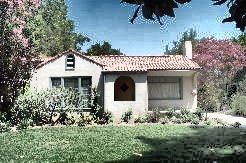
\includegraphics[width=0.45\textwidth]{./Figures/calhouse_236/101-resultado.jpg}
}
    % \begin{subfigure}[t]{0.45\textwidth}
        %\caption{Enhanced Image using \cite{morepso}. $\mathscr{H_Y}=0.788927$. $SSIM_R=0.000204143$. $SSIM_G=0.0000526475$. $SSIM_B=0.0000518143$}
        % \label{fig:calhouse23129}
        \end{subfigure}
    ~ %add desired spacing between images. e. g. ~. \quad. \qquad. \hfill etc. 
    %(or a blank line to force the subfigure onto a new line)
    \begin{subfigure}[ID=56]{
    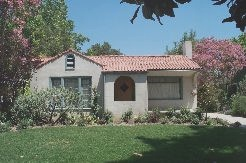
\includegraphics[width=0.45\textwidth]{./Figures/calhouse_236/107-resultado.jpg}
    }
    % \begin{subfigure}[t]{0.45\textwidth}
%        \caption{Enhanced Image.  $\mathscr{H_Y}=0.0350595$. $SSIM_R=0.416776$. $SSIM_G=0.403636$. $SSIM_B=0.417654$}
% \label{fig:calhouse231102}
\end{subfigure} 
\begin{subfigure}[Imagen Original]{
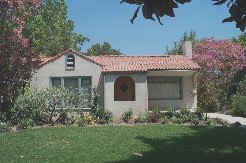
\includegraphics[width=0.45\textwidth]{./Figures/calhouse_236/calhouse_236.jpg}
}
    % \begin{subfigure}[t]{0.45\textwidth}
        %\caption{Enhanced Image using \cite{morepso}. $\mathscr{H_Y}=0.788927$. $SSIM_R=0.000204143$. $SSIM_G=0.0000526475$. $SSIM_B=0.0000518143$}
        % \label{fig:calhouse233orig}
        \end{subfigure}
        \caption{Imágenes visualmente relevantes obtenidas mediante $CMOPSO-CLAHE$. Las variables y decisión y métricas de las imágenes se muestran en la tabla \ref{tab:calhouse_234}.}
        \label{fig:anexocalhouse236}
        \end{figure}

        \begin{figure}[H]
        \centering
        %\begin{subfigure}[Gráfica de Frente Pareto para las soluciones no dominadas de \texttt{calhouse_231.jpg}]{
        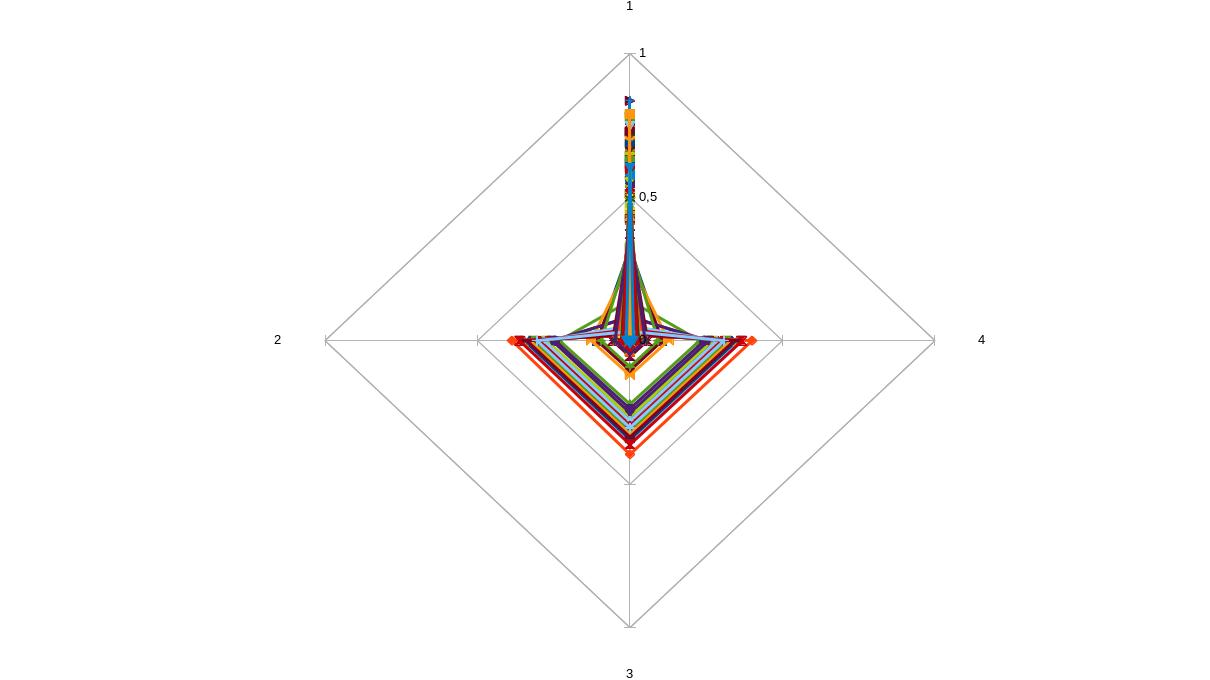
\includegraphics[width=\textwidth]{./Figures/calhouse_236/calhouse_236_2.jpg}
        %}
        %\end{subfigure}
        \caption{Frente pareto que contrasta los objetivos de las soluciones no dominadas. para los resultados de imágenes que se muestran en la tabla \ref{tab:calhouse_236}.}
        \label{fig:calhouse2362fp}
        \end{figure}



\section{Imagen de prueba \texttt{calhouse\_237.jpg}}

%calhouse 234
\scriptsize
\begin{longtable}{|c|c|c|c|c|c|c|c|}
% \centering
%\begin{tabular}
\hline
ID & $\mathscr{R}_x$ & $\mathscr{R}_y$ & $\mathscr{C}$ & $f_1(I.\vv{x})$ & $f_2(I.\vv{x})$ & $f_3(I.\vv{x})$ & $f_4(I.\vv{x})$ \\
\hline

\multicolumn{8}{|c|}{\textbf{Tiempos de ejecución:} \texttt{
}}\\  \hline
% \end{tabular}
\caption{Resultados no dominados para la imagen de prueba \texttt{calhouse\_237.jpg}}
\label{tab:calhouse_237}
\end{longtable}
\normalsize

\begin{figure}[H]
\centering
    %\begin{subfigure}[t]{0.45\textwidth}
    \begin{subfigure}[ID=0]{
    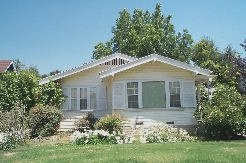
\includegraphics[width=0.45\textwidth]{./Figures/calhouse_237/9048-resultado.jpg}
    }
%        \caption{Imagen Original. $\mathscr{H_Y}=0.207231$. $SSIM_R=1$. $SSIM_G=1$. $SSIM_B=1$}
\end{subfigure}
    ~ %add desired spacing between images. e. g. ~. \quad. \qquad. \hfill etc. 
      %(or a blank line to force the subfigure onto a new line)
      \begin{subfigure}[ID=1]{
      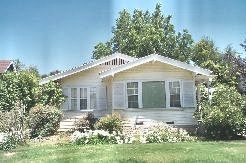
\includegraphics[width=0.45\textwidth]{./Figures/calhouse_237/9090-resultado.jpg}   
      }
    %\begin{subfigure}[t]{0.45\textwidth}
%        \caption{Enhanced Image. $\mathscr{H_Y}=0.611275$. $SSIM_R=0.00897331$. $SSIM_G=0.00823064$. $SSIM_B=0.00851013$}
\end{subfigure}
    ~ %add desired spacing between images. e. g. ~. \quad. \qquad. \hfill etc. 
    %(or a blank line to force the subfigure onto a new line)
    \begin{subfigure}[ID=23]{
    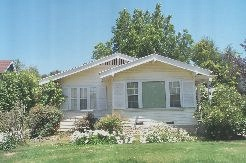
\includegraphics[width=0.45\textwidth]{./Figures/calhouse_237/9095-resultado.jpg}
    }
    % \begin{subfigure}[t]{0.45\textwidth}
%        \caption{Enhanced Image.  $\mathscr{H_Y}=0.0350595$. $SSIM_R=0.416776$. $SSIM_G=0.403636$. $SSIM_B=0.417654$}
\end{subfigure} 
\begin{subfigure}[ID=24]{
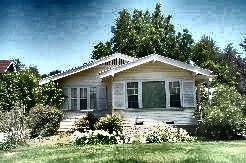
\includegraphics[width=0.45\textwidth]{./Figures/calhouse_237/9162-resultado.jpg}
}
    % \begin{subfigure}[t]{0.45\textwidth}
        %\caption{Enhanced Image using \cite{morepso}. $\mathscr{H_Y}=0.788927$. $SSIM_R=0.000204143$. $SSIM_G=0.0000526475$. $SSIM_B=0.0000518143$}
        % \label{fig:calhouse23129}
        \end{subfigure}
    ~ %add desired spacing between images. e. g. ~. \quad. \qquad. \hfill etc. 
    %(or a blank line to force the subfigure onto a new line)
    \begin{subfigure}[ID=56]{
    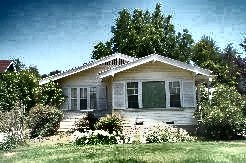
\includegraphics[width=0.45\textwidth]{./Figures/calhouse_237/9175-resultado.jpg}
    }
    % \begin{subfigure}[t]{0.45\textwidth}
%        \caption{Enhanced Image.  $\mathscr{H_Y}=0.0350595$. $SSIM_R=0.416776$. $SSIM_G=0.403636$. $SSIM_B=0.417654$}
% \label{fig:calhouse231102}
\end{subfigure} 
\begin{subfigure}[Imagen Original]{
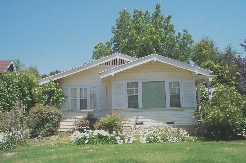
\includegraphics[width=0.45\textwidth]{./Figures/calhouse_237/calhouse_237.jpg}
}
    % \begin{subfigure}[t]{0.45\textwidth}
        %\caption{Enhanced Image using \cite{morepso}. $\mathscr{H_Y}=0.788927$. $SSIM_R=0.000204143$. $SSIM_G=0.0000526475$. $SSIM_B=0.0000518143$}
        % \label{fig:calhouse233orig}
        \end{subfigure}
        \caption{Imágenes visualmente relevantes obtenidas mediante $CMOPSO-CLAHE$. Las variables y decisión y métricas de las imágenes se muestran en la tabla \ref{tab:calhouse_237}.}
        \label{fig:anexocalhouse237}
        \end{figure}

        \begin{figure}[H]
        \centering
        %\begin{subfigure}[Gráfica de Frente Pareto para las soluciones no dominadas de \texttt{calhouse_231.jpg}]{
        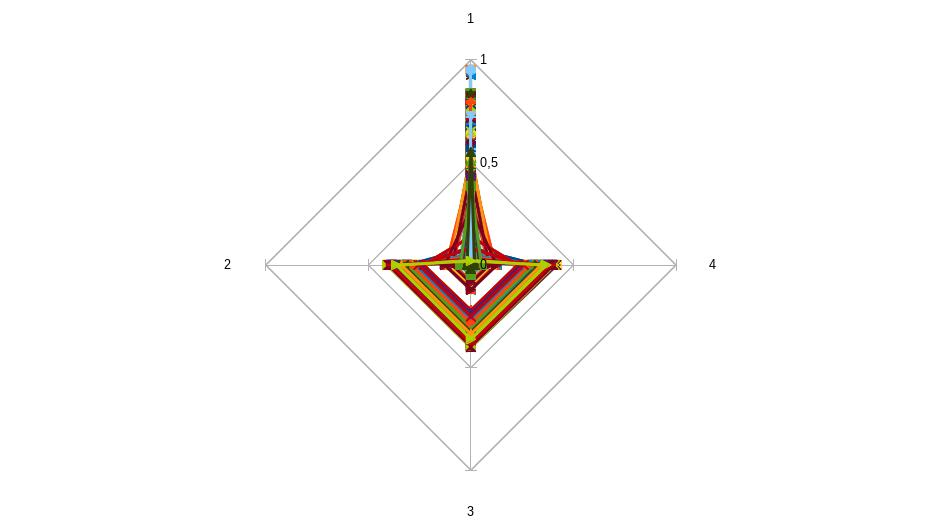
\includegraphics[width=\textwidth]{./Figures/calhouse_237/calhouse_237_2.jpg}
        %}
        %\end{subfigure}
        \caption{Frente pareto que contrasta los objetivos de las soluciones no dominadas. para los resultados de imágenes que se muestran en la tabla \ref{tab:calhouse_237}.}
        \label{fig:calhouse2372fp}
        \end{figure}        
% \begin{table}[H]
% \centering
% \caption{Promedios de los tiempos de ejecución de algoritmo HE para las imágenes en escala de grises.}
% \label{tabla22}
% \begin{tabular}{|c|c|}
% \hline
% \begin{tabular}[c]{@{}c@{}}Nº de \\ ejecución\end{tabular} & \begin{tabular}[c]{@{}c@{}}t\\ (ms)\end{tabular} \\ \hline
% 1                                                          & 1.145                                            \\
% 2                                                          & 0.945                                            \\
% 3                                                          & 0.97                                             \\
% 4                                                          & 0.925                                            \\
% 5                                                          & 0.95                                             \\ \hline
% Promedio                                                   & \textbf{0.987}                                   \\ \hline
% \end{tabular}
% \end{table}


% En la Tabla \ref{tabla23} se muestran los promedios de los tiempos de ejecución del algoritmo MMCE para las imágenes en escala de grises.

% % Please add the following required packages to your document preamble:
% % \usepackage{multirow}
% \begin{table}[H]
% 	\centering
% 	\caption{Promedios de los tiempos de ejecución del algoritmo MMCE para las imágenes en escala de grises.}
% 	\label{tabla23}
% 	\begin{tabular}{|c|c|c|c|c|c|c|}
% 		\hline
% 		\multirow{2}{*}{Iter. (n)} & \multicolumn{5}{c|}{Nº de ejeciciones para el algoritmo MMCE} & \multirow{2}{*}{\begin{tabular}[c]{@{}c@{}}Promedios\\ t(ms)\end{tabular}} \\ \cline{2-6}
% 		& 1           & 2          & 3         & 4         & 5          &                                                                            \\ \hline
% 		1                          & 64.265      & 62.625     & 61.61     & 62.285    & 62.295     & \textbf{62.616}                                                            \\
% 		2                          & 165.805     & 171.24     & 169.655   & 170.515   & 170.295    & \textbf{169.502}                                                           \\
% 		3                          & 327.975     & 334.19     & 334.75    & 332.045   & 333.275    & \textbf{332.447}                                                           \\
% 		4                          & 564.035     & 574.15     & 571.185   & 573.45    & 568.735    & \textbf{570.311}                                                           \\
% 		5                          & 975.845     & 972.035    & 979.205   & 968.975   & 986.805    & \textbf{976.573}                                                           \\
% 		6                          & 1454.415    & 1471.145   & 1449.78   & 1452.97   & 1463.74    & \textbf{1458.41}                                                           \\
% 		7                          & 2037.11     & 2032.775   & 2041.54   & 2029.07   & 2038.735   & \textbf{2035.846}                                                          \\ \hline
% 	\end{tabular}
% \end{table}


% En la Tabla \ref{tabla24} se muestran los promedios de los tiempos de ejecución del algoritmo propuesto para las imágenes en escala de grises.

% % Please add the following required packages to your document preamble:
% % \usepackage{multirow}
% \begin{table}[H]
% 	\centering
% 	\caption{Promedios de los tiempos de ejecución del algoritmo propuesto para las imágenes en escala de grises.}
% 	\label{tabla24}
% 	\begin{tabular}{|c|c|c|c|c|c|c|}
% 		\hline
% 		\multirow{2}{*}{Iter. (n)} & \multicolumn{5}{c|}{Nº de ejeciciones para el algoritmo propuesto} & \multirow{2}{*}{\begin{tabular}[c]{@{}c@{}}Promedios \\ t(ms)\end{tabular}} \\ \cline{2-6}
% 		& 1            & 2           & 3           & 4          & 5          &                                                                             \\ \hline
% 		1                          & 62.105       & 63.055      & 61.99       & 62.445     & 62.955     & 62.51                                                                       \\
% 		2                          & 166.74       & 169.645     & 168.34      & 168.435    & 169.34     & 168.5                                                                       \\
% 		3                          & 327.175      & 332.58      & 331.765     & 332.755    & 331.52     & 331.159                                                                     \\
% 		4                          & 565.245      & 576.84      & 574.47      & 573.6      & 572.15     & 572.461                                                                     \\
% 		5                          & 976.57       & 973.22      & 968.35      & 970.245    & 975.26     & 972.729                                                                     \\
% 		6                          & 1463.175     & 1474.82     & 1458.765    & 1459.83    & 1470.06    & 1465.33                                                                     \\
% 		7                          & 2047.435     & 2040.82     & 2041.915    & 2039.95    & 2044.16    & 2042.856                                                                    \\ \hline
% 	\end{tabular}
% \end{table}

